\documentclass[12pt, letterpaper]{paper}
\usepackage[utf8]{inputenc}
\usepackage[T1]{fontenc}
\usepackage{graphicx}
\usepackage{grffile}
\usepackage{longtable}
\usepackage{wrapfig}
\usepackage{rotating}
\usepackage[normalem]{ulem}
\usepackage{textcomp}
\usepackage{amssymb}
\usepackage{capt-of}
\usepackage{hyperref}
\usepackage{tikz}
\usepackage{Schwieg}

\usetikzlibrary{patterns}



\author{Timothy Schwieg}
\date{\today}
\title{Rudin Notes}


\hypersetup{ pdfauthor={Timothy Schwieg}, pdftitle={Rudin Notes},
  pdfkeywords={}, pdfsubject={}, pdfcreator={Timothy Schwieg}, pdflang={English}}

\begin{document}

\maketitle

\section{Chapter 1}
\label{sec:orge957eb3}


\subsection{Real Numbers}
\label{sec:org8f023da}
Rational Numbers are not quite descriptive enough:

There is no rational number p such that: $p^2 = 2$
\begin{proof}
  Approach by Contradiction:

  $p = \frac{m}{n}$ where m,n are irreducible integers. Then:
  $m^2 = 2 n^2$.  Thus $m^2$ is even, and therefore $m$ is even. So
  $m^2$ is divisible by $4$.  This means $2n^2$ is divisible by 4, and
  $n^2$ is even, so n is even. Contradiction.
\end{proof}

The point of the real numbers is to introduce a set of numbers that
fills in these "gaps" and arises from the concepts of an ordered set
and a field. As we can see later, the rational numbers are not
complete, and do not satisfy some very important properties required
for analysis.

For a set S, an order on S is a relation, denoted $<$.

\begin{enumerate}
\item If $x \in S$ and $y \in S$ then one of these is true:
  $x < y, x = y, y < x$
\item If $x,y,z \in S$, $x < y, y < z, \implies x < z$.
\end{enumerate}


Ordered Set: An ordered Set is a set where there is a defined order.

If S is an ordered Set, and $E \subset S$, if
$\exists \beta \in S, x \leq \beta \quad \forall x \in E$, E is
bounded above with upper bound $\beta$.

\vspace{ .33in }

Least Upper Bound (supremum): For an ordered set S, $E \subset S$
where E is bounded above. If $\exists \alpha \in S$
\begin{itemize}
\item $\alpha$ is an upper bound of E
\item $\forall \gamma < \alpha$, $\gamma$ is not an upper bound of E.
\end{itemize}
This is denoted: $\alpha = \sup{ E }$, The infimum of a set, denoted
$\delta = \inf{ E}$ is defined in a similar manner.

\vspace{ .33in }

The supremum of a set need not be contained within that set. Consider
the set containing numbers of the form:
$\frac{1}{N}, n \in \mathbb{Z^{++}}$. The sup of this set is 1, which
is contained, but the inf of the set is 0, and is not contained within
the set.

\vspace{ .33in }

Least-Upper-Bound property: The supremum of every nonempty subset is
contained in the original set.
\begin{itemize}
\item $E \subset S \neq \emptyset$.
\item $E$ is bounded above
\item $\sup{E}$ exists in S.
\end{itemize}

Having the Least-Upper-Bound Property implies that you also have the
Greatest-Lower-Bound Property:

\begin{theorem}
  % Relationship between sup and inf
  \label{thr:1.11}
  If S is an ordered set with least-upper-bound property,
  $B \subset S, B \neq \emptyset$ and B is bounded below, let L be the
  set of all lower bounds of B. Then $\alpha = \sup{L} \in S$, and
  $\alpha = \inf{B}$.
\end{theorem}
\begin{proof}
  B is bounded below, so there is at least one element as a lower
  bound, and L is nonempty. L is all the lower bounds, so any element
  in B is an upper bound on L. This means L is bounded above, and thus
  L has a supremum contained in S. $\alpha = \sup{L} \in S$.

  Since $\alpha$ is the least upper bound of L, any number
  $\gamma < \alpha$ is not an upper bound of L. Therefore
  $\gamma \notin B$ as if it were, $\delta > \gamma \in L$ could not
  be a lower bound of $B$. This means that
  $\forall x \in B, \quad \gamma < x$. Then $\alpha \leq x$. If this
  were not true: Let $\epsilon = \alpha - x > 0$. Choose
  $\gamma = \alpha - \frac{\epsilon}{2}$. Then $\gamma > x$ but this
  is an impossibility.  Since $\alpha$ is an upper bound on L, any
  number larger than it cannot be contained in the set. Since
  $\alpha \in L$ it is a lower bound of B, but any number larger than
  it is not a lower bound, so it must be that: $\alpha = \inf{B}$.
\end{proof}


Field: Set F with two operations that satisfy the following "field
axioms".

(A) Axioms for addition
\begin{itemize}
\item If $x \in F$ and $y \in F$, then $x + y \in F$.
\item $\forall x,y \in F \quad x + y = y + x$
\item $\forall x,y,z \in F \quad ( x + y ) + z = x + (y+z)$
\item $\exists0 \in F$ such that: $0 + x = x$
\item $\forall x \in F, \exists -x$ such that: $x + (-x) = 0$
\end{itemize}

(M) Axioms for Multiplication
\begin{itemize}
\item If $x \in F$ and $y \in F$ then their product $xy \in F$
\item $\forall x,y \in F, xy = yx$
\item $\forall x,y,z \in F, (xy)z = x(yz)$
\item $\exists 1 \in F$ such that: $1x = x$
\item $\forall x \in F, x \neq 0 \quad \exists \frac{1}{x} \in F$ such
  that: $x (\frac{1}{x}) = 1$
\end{itemize}

Distributive law:
\begin{itemize}
\item $\forall x,y,z \in F, x(y+z) = xy + xz$
\end{itemize}

\vspace{ .33in }

The axioms above imply the following statements:
\begin{itemize}
\item $x+y = x+z \to y = z$
\item $x + y = x \to y = 0$
\item $x+y = 0 \to x = -y$
\item $-(-x) = x$
\end{itemize}

\begin{proof} This is filler\newline
  \begin{itemize}
  \item $x + y = x + z$ \newline $(-x) + x + y = (-x) + x + z$
    \newline $( -x + x ) + y = (-x + x ) + z$\newline $y = z$
  \item Let z = 0 above.
  \item
    $x+y = 0 \to (-x) + x + y = -x \implies (-x + x) + y = -x \to y =
    -x$
  \item
    $-(-x) + (-x) = 0 \implies -(-x) + (-x) = x + -x \to -(-x) = x$
  \end{itemize}
\end{proof}

Basically, cancellation laws hold, and the zero element in unique as
well as the additive inverse of any element.

Similarly for multiplication: Note $x\neq0$ for all results
\begin{itemize}
\item $xy = xz \implies y = z$
\item $xy = x \implies y = 1$
\item $xy = 1 \implies y = \frac{1}{x}$
\item $\frac{1}{\frac{1}{x}} = x$
\end{itemize}

\vspace{ .33in }

We also Get:
\begin{itemize}
\item $0x = 0$
\item If $x \neq0, y\neq0$, then $xy \neq 0$
\item $(-x)y = -(xy) = x(-y)$
\item $(-x)(-y) = xy$
\end{itemize}

Proof:
\begin{itemize}
\item $0x = (-x + x )x = -x^2 + x^2 = 0$
\item Assume $xy =0$. Then $xy \frac{1}{y} = 0 \frac{1}{y}$. By result
  above: $x = 0$ which is a contradiction.
\item $-xy = xy - xy - xy = y( x -x -x ) = y( -x )$ \newline
  $-xy = xy - xy - xy = x( y - y -y ) = x(-y)$
\item $(-x)(-y) = -(x(-y)) = -( - (xy ) ) = xy$
\end{itemize}

\begin{enumerate}
\item Ordered Field
  \label{sec:org4b78c5c}
  Ordered Field: A field F for which there is also an ordered set that
  satisfies:
  \begin{itemize}
  \item $x + y < x + z$ if: $x,y,z \in F$ and $y<z$
  \item $xy > 0$ if $x \in F, y \in F, x >0, y >0$
  \end{itemize}

  Useful results in ordered Fields:
  \begin{itemize}
  \item If $x > 0$ then $-x < 0$
  \item If $x > 0$ and $y < z$ then $xy < xz$
  \item If $x < 0$ and $y < z$ then $xy > xz$
  \item If $x \neq 0$ then $x^2 > 0$, so $1 > 0$
  \item If $0 < x < y$ then $0 < \frac{1}{y} < \frac{1}{x}$
  \end{itemize}

  Proof:
  \begin{itemize}
  \item $x > 0 \to x + (-x) > -x \to 0 > -x$
  \item $y < z \to z-y > 0 \to x(z-y) > 0 \to zx > xy$
  \item Repeat using -x
  \item $^{}x^{2} = xx = (-x)(-x)$ One of which is the product of two
    positive numbers. Thus $x^{2} > 0$.
  \item
    $x < y \to x \frac{1}{x} < y \frac{1}{x} \to \frac{1}{y} <
    \frac{1}{x}$
  \end{itemize}
  \vspace{ .33in }
\end{enumerate}

\begin{theorem}
  % Completeness Axiom
  \label{thr:1.19}
  There exists an ordered field $\setR$ which has the
  least-upper-bound property.  $\setR$ contains $\setQ$ as a
  sub-field.
\end{theorem}

\begin{theorem}
  % Archimedian Property and density of rationals
  \label{thr:1.20}
  \begin{enumerate}
  \item Archimedian Property: If $x > 0$ and $x,y \in \setR$, then
    $\exists n \in \setZ$ such that: $nx > y$
  \item $\setQ$ is dense in $\setR$: $x,y \in \setR, x < y$ implies
    that $\exists p \in \setQ$ such that: $x < p < y$.
  \end{enumerate}
\end{theorem}
\begin{proof}
  \begin{enumerate}
  \item Let A be the set of all $nx$ where $n \in \setZ^{++}$. Assume
    the result is false, A is bounded above by y. A must have a
    supremum, let $\alpha = \sup{A}$. Note that: $\alpha - x < \alpha$
    so $\alpha - x$ is not an upper bound for A. So there is an
    integer $m$ such that $\alpha - x < mx$.  However, this implies:
    $\alpha < (m+1)x$ This is a contradiction since $\alpha$ is an
    upper bound of A.
  \item Note: $y-x > 0$. By the Archimedian property: $n(y-x) > 1$.
    $m_{1} > nx, m_2 > -nx$. This means that: $-m_2 < nx < m_1$. Since
    $nx$ is bounded by two integers, there is a single integer $m$
    such that: $m-1 \leq nx < m$. Combining all these results:
    \newline $nx < m \leq 1 + nx < ny \to x < \frac{m}{n} < y$.
  \end{enumerate}
  
\end{proof}

Some simple corollaries from this that can be created are: For any
real number $x$ there is an integer $N$ such that $\frac{1}{N} < x$.


\begin{theorem}
  % uniqueness of $y^n = x$
  \label{thr:1.21}
  For every real $x>0$ and integer $n > 0$ there is only one positive
  real y such that $y^{n} = x$
\end{theorem}
\begin{proof}
  Assume there are multiple distinct y values satisfying it: WLOG
  consider $y_1 < y_2$ Note then that: $y_1^n < y_2^n$ and they cannot
  be equal.  \newline Let us consider the existence now. Let the set
  $E$ contain all positive real numbers $t$ such that: $t^n < x$. Note
  that $E$ always contains: $\frac{x}{1+x}$, as this is less than one,
  and $t^n \leq t < x$. This ensures E is not empty.

  $1+x$ is an upper bound of t, as $t>1+x \to t > x$ and $t^n \geq
  t$. This means that E has a least upper bound.

  Let $y = \sup{E}$. The book then follows some nasty algebraic
  identities to draw contradictions around $y^n > x$ and $y^n < x$ and
  then asserts that $y^n = x$.
\end{proof}

Extended Real Numbers: Real numbers with $\infty$ and $-\infty$ added
to them. This still preserves the original ordering in $\setR$. We
declare that: $-\infty < x < \infty \quad \forall x \in \setR$.

This provides an upper and lower bound to every subset of the extended
reals, so as long as the subset is nonempty it will always have a
least-upper-bound and a greatest-lower-bound. We are no longer a
field, but we simply define the usual conventions with infinity.

\subsection{Complex Field}
\label{sec:org27d8085}
A Complex number is an ordered pair of real numbers. For two complex
numbers, $x = (a,b), y = (c,d)$, Addition and Multiplication are
defined as such:

\begin{align*}
  x+y &= (a+c,b+d)\\
  xy &= (ac-bd, ad+bc )\\
\end{align*}

These definitions ensure that the set of all complex numbers is a
field, where $0 = (0,0)$ and $1 = (1,0)$. The axioms are then verified
in the book.

One useful way to think about the complex numbers is as an extension
of the real numbers, where the second ordered pair is equal to
zero. All operations under the complex numbers follow the same
properties.

We can now define the imaginary constant: $i = (0,1)$. This is the
number with the property: $i^{2} = -1$. For two real numbers
$a,b; (a,b)= a + b i$.

We define the \emph{Conjugate} of a complex number $z = a+b i$ to be:
$\conj{z} = a - b i$. For notational sake, define:
$a = Re(z), b = Im(z)$

\begin{theorem}
  % Conjugate Properties
  \label{thr:1.31}
  \begin{enumerate}
  \item $\conj{z+w} = \conj{z} + \conj{w}$
  \item $\conj{zw} = \conj{z} \conj{w}$.
  \item $z + \conj{z} = 2 Re(z)$
  \item $z - \conj{z} = 2i Im(z)$
  \item $z \conj{z}$ is real and positive, or zero if $z = (0,0)$
  \end{enumerate}
\end{theorem}



The Absolute value of a complex number: $\abs{z}$. is the square root
of $z \conj{z}$. $\abs{z} = ( z \conj{z} )^{\frac{1}{2}}$ This number
is unique and exists (from theorem \ref{thr:1.21}). For real numbers
this carries the traditional view of absolute value.

\begin{theorem}
  % Absolute value properties
  \label{thr:1.33}
  \begin{enumerate}
  \item $\abs{z} > 0$ unless $z = 0, \abs{0} = 0$
  \item $\abs{\conj{z}} = \abs{z}$
  \item $\abs{zw} = \abs{z}\abs{w}$
  \item $\abs{Re(z)} \leq \abs{z}$
  \item $\abs{z+w} \leq \abs{z} + \abs{w}$
  \end{enumerate}
\end{theorem}

\begin{proof}
  \begin{enumerate}
  \item Follows directly from: $z \conj{z} > 0$ for $z \neq 0$
  \item
    $\abs{\conj{z}} = ( a^{}2 + (-b)^{2} )^{\frac{1}{2}} = ( a^{2} +
    b^{2})^{}\frac{1}{2} = \abs{z}$
  \item
    $\abs{zw}^2 = (ac-bd)^2 + (ad+bc)^2 = (a^2 + b^2 )(c^2 + d^2) =
    \abs{z}^2 \abs{w}^2 = (\abs{z}\abs{w})^{2}$
  \item
    $\abs{Re(z)} = \sqrt{ a^{2} } \leq \sqrt{ a^{2} + b^{2} } =
    \abs{z}$
  \item
    $\abs{z+w}^{2} = z \conj{z} + z \conj{w} + \conj{z}w + w \conj{w}$
    \newline $= \abs{z}^2 + 2 Re( z \conj{w} ) + \abs{w}^{2}$ \newline
    $\leq \abs{z}^{2} + 2\abs{z \conj{w} } + \abs{w}^{2}$ \newline
    $= ( \abs{z} + \abs{w} )^{2}$
  \end{enumerate}
\end{proof}


\begin{theorem}
  % Schwarz inequality
  \label{thr:1.35}
  Let $a_{1} ... a_{n}$ be complex numbers, and $b_{1} ... b_{n}$ be
  complex numbers.

\begin{align*}
  \abs{ \sum_{j=1}^n a_j \conj{b_j} }^2 \leq \sum_{j=1}^n \abs{a_j}^2 \sum_{j=1}^n \abs{b_j}^2
\end{align*}
\end{theorem}
\begin{proof}
  Let
  $A = \sum \abs{ a_j }^2, B = \sum \abs{ b_j }^2 , C = \sum a_j
  \conj{b_j}$. Note that if $B = 0$ then the result is trivial, let
  $B > 0$.
  \begin{align*}
    \sum \abs{ B a_j - C b_j }^2 &= \sum ( B a_j - C b_j )( B \conj{a_j} - \conj{C b_j} )\\
                                 &= B^2 \sum \abs{a_j}^2 - B \conj{C} \sum a_j \conj{b_j} - BC \sum \conj{a_j} b_j + \abs{C}^2 \sum \abs{b_j}^2 \\
                                 &= B^2 A - B \abs{C}^2 \\
                                 &= B( AB - \abs{C}^2 ) \geq 0\\
  \end{align*}
  Since it is known that $B > 0$ then we get $AB - \abs{C}^2 \geq 0$.
\end{proof}


\subsection{Euclidean Spaces}
\label{sec:orgd268d85}
For a positive integer k, $\setR^{k}$ is the set of of all ordered
k-tuples. Elements in this space are called vectors, and denoted by
boldface letters. Vector addition and scalar multiplication are
defined as such:

\begin{align*}
  \vec{x} + \vec{y} &= ( x_1 + y_1, ..., x_k + y_k )\\
  \alpha \vec{x} &= ( \alpha x_1, ..., \alpha x_k )\\
\end{align*}
These operations are closed, and make $\setR^{k}$ into a vector space
over the real field. The zero element in this space is the point
$\vec{0}$, whose coordinates are all $0$.

The inner-product of two vectors as well as the norm is defined as:
\begin{align*}
  \vec{x} \cdot \vec{y} &= \sum_{i=1}^k x_i y_i \\
  \abs{\vec{x}} &= \left( \sum_{i=1}^k x_i^2 \right )^{\frac{1}{2}} \\
\end{align*}

\begin{theorem}
  % Norm Properties
  \label{thr:1.37}
  For $\vec{x}, \vec{y}, \vec{z} \in \setR^{k}, \alpha \in \setR$
  \begin{enumerate}
  \item $\abs{\vec{x}} \geq 0$
  \item $\abs{\vec{x}} = 0 \Leftrightarrow \vec{x} = 0$
  \item $\abs{\alpha \vec{x}} = \abs{\alpha} \abs{\vec{x}}$
  \item
    $\abs{ \vec{x} \cdot \vec{y} } \leq \abs{\vec{x} } \abs{\vec{y}}$
  \item $\abs{ \vec{x} + \vec{y} } \leq \abs{\vec{x}} + \abs{\vec{y}}$
  \end{enumerate}
\end{theorem}

\begin{proof}
  \begin{enumerate}
  \item Follows directly from the definition of $\abs{\vec{x}}$
  \item If $\vec{x} = 0, x_{i} = 0 \quad \forall i$. So
    $\sum x_{i}^{2} = 0$. If $\vec{x} \neq 0, x_{i} \neq 0$ for some
    i. $x_{i}^{2} > 0$ for at least one element i, and
    $\sum_{ }x_{i}^{2} > 0$.
  \item
    $\abs{\alpha \vec{x}} = ( \alpha \vec{x} \cdot \alpha \vec{x}
    )^{}{\frac{1}{2}} = \abs{\alpha} \abs{ x }$
  \item
    $\abs{ \vec{x} \cdot \vec{y} } = \abs{ \sum x_{i} y_{i} } \leq
    \left ( \sum \abs{x_{i}}^2 \sum \abs{y_{i}}^{2} \right
    )^{\frac{1}{2}} = \abs{\vec{x}} \abs{\vec{y}}$
  \item
    $\abs{ \vec{x} + \vec{y}}^{2} = (\vec{x} + \vec{y}) \cdot (\vec{x}
    + \vec{y})$ \newline
    $= \vec{x} \cdot \vec{x} + 2\vec{x} \cdot \vec{y} + \vec{y} \cdot
    \vec{y}$ \newline
    $\leq \abs{\vec{x}}^{2} + 2 \abs{\vec{x}} \abs{\vec{y}} +
    \abs{\vec{y}}^2$ \newline $= ( \abs{x} + \abs{y} )^2$
  \end{enumerate}
\end{proof}

\vspace{ .33in }

\subsection{Exercises}
\label{sec:org4a96c4c}
\subsubsection{Question 1}
\label{sec:org9e9c36f}
\begin{question}
  If r is rational and not equal to zero, and x is irrational, prove
  that r+x and rx are irrational
\end{question}
\begin{proof}
  Let r+x be rational, then it can be written as a fraction of
  irreducible integers: $r+x = \frac{m}{n}$. Since r is rational, it
  can be written as $r = \frac{a}{b}$.  Therefore x can be written as:
  $x = \frac{m}{n} - \frac{a}{b} = \frac{bm - an}{nb}$ This is a
  contradiction to x being irrational.

  Let rx be rational. $rx = \frac{m}{n}$. Since r is rational it can
  be written as $r = \frac{a}{b}$.  Then
  $x = \frac{\frac{m}{n}}{\frac{a}{b}} = \frac{mb}{an}$ which is again
  a contradiction
\end{proof}

\subsubsection{Question 2}
\label{sec:org534551b}
\begin{question}
  Prove that there is no rational number whose square is 12
\end{question}
\begin{proof}
  Assume there is a rational number with square 12.
  $x = \frac{m}{n}, x^2 = 12$.  $\frac{m^2}{n^2} = 12, m^2 = 12n^2$
  This implies $m^2$ is divisible by 12.  Assume m is not divisible by
  six. Then: $m = 6l + w$ and $m^2 = 36l^2 + 12lw + w^2$.  Note that
  $w^2$ is not divisible by six for $w = \{1,2,3,4,5\}$.  $m$ is
  divisible by six. So $m^2 = 36k, 12n^2 = 36k$. Thus $n^2$ is
  divisible by 3.  Assume $n$ is not divisible by three. Then
  $n = 3l + w$ and $n^2 = 9l + 6lw + w^2$.  Note that $w^2$ is not
  divisible by three for $w = \{1,2\}$.  $n$ is divisible by three,
  and $m,n$ have a common factor, leading to a contradiction.
\end{proof}

\subsubsection{Question 3}
\label{sec:org1c15d6f}
Ommitted because of how trivial it is.

\subsubsection{Question 4}
\label{sec:orgc442add}
\begin{question}
  Let E be a nonempty subset of an ordered set; suppose $\alpha$ is a
  lower bound of E, and $\beta$ is an upper bound of E. Prove that
  $\alpha \leq \beta$.
\end{question}
\begin{proof}
  Case: E is a singleton set. Let x be an element in E. Then
  $\alpha \leq x$ and $x \leq \beta$. So $\alpha \leq \beta$.
\end{proof}

\subsubsection{Question 5}
\label{sec:orgfaec5fd}
\begin{question}
  Let A be a nonempty set of real numbers which is bounded below. Let
  $-A$ bet he set of all numbers $-x$ where $x \in A$. Prove that:
  $\inf{A} = - \sup( -A )$.
\end{question}
\begin{proof}
  Let $\alpha = \inf{A}$. Then $\forall x \in A, \alpha \leq x$ and
  $\alpha + \epsilon$ is not an lower bound:
  $\exists y \in A, y < \alpha + \epsilon$.  So: $-\alpha \geq -x$ and
  $-\alpha - \epsilon < y \quad \forall\epsilon > 0$. This means that
  $-\alpha$ is the least upper bound for $-A$.
\end{proof}


\subsubsection{Question 8}
\label{sec:org2ae56a0}
\begin{question}
  Prove that no order can be defined in the complex field that turns
  it into a an ordered field.
\end{question}
\begin{proof}
  Assume that there is an order in the complex field: Note that this
  implies $1 > 0$.  This means that $-1 < 0$ and for any
  $x \neq 0, x^2 > 0$. Take $x = i$. $i^2 = -1$ which is a
  contradiction.
\end{proof}

\subsubsection{Question 12}
\label{sec:org80a6e23}
\begin{question}
  If $z_1 , ... , z_n$ are complex, prove that:
  $\abs{ z_1 + z_2 + ... + z_n } \leq \abs{ z_1 } + ... + \abs{z_n}$
\end{question}
\begin{proof}
  By Induction.  Base Case: n = 1. $\abs{ z_1 } = \abs{z_1}$. \newline
  Inductive Step:
  $\abs{ z_1 + ... z_{k-1} + z_k } \leq \abs{ z_1 + ... + z_{k-1} } +
  \abs{z_k } \leq \abs{ z_1 } + ... + \abs{ z_{k-1} } + \abs{z_k}$.
  The first step uses the triangle inequality, and the second uses the
  induction hypothesis.
\end{proof}

\subsubsection{Question 13}
\label{sec:org654cb1f}
\begin{question}
  If $x,y \in \mathbb{C}$, prove that:
  $\abs{ \abs{x} - \abs{y} } \leq \abs{x - y}$
\end{question}
\begin{proof}
  \begin{align*}
    \abs{ \abs{x} - \abs{y} } &= \abs{ \abs{x - y + y } - \abs{y} } \\
                              &\leq \abs{ \abs{ x - y } + \abs{y} - \abs{y} } = \abs{ x - y}
  \end{align*}
\end{proof}


\subsubsection{Question 17}
\label{sec:orgb1daeda}
\begin{question}
  Prove that:
  \begin{align*}
    \abs{\vec{x}+\vec{y}}^2 + \abs{\vec{x} - \vec{y}}^2 = 2\abs{\vec{x}}^2 + 2\abs{\vec{y}}^2
  \end{align*}
\end{question}
\begin{proof}
  \begin{align*}
    \abs{\vec{x}+\vec{y}}^2 + \abs{\vec{x} - \vec{y}}^2 &= (\vec{x} + \vec{y} )\cdot(\vec{x} + \vec{y}) + (\vec{x} - \vec{y})\cdot(\vec{x}-\vec{y})\\
                                                        &= \vec{x}\cdot \vec{x} + 2 \vec{x} \cdot \vec{y} + \vec{y} \cdot \vec{y} + \vec{x} \cdot \vec{x} - 2 \vec{x} \cdot \vec{y} + \vec{y} \cdot \vec{y}\\
                                                        &= 2 \vec{x} \cdot \vec{x} + 2 \vec{y} \cdot \vec{y} \\
                                                        &= 2 \abs{ \vec{x} }^2 + 2 \abs{ \vec{y} }^2\\
  \end{align*}
\end{proof}

\section{Basic Topology}
\label{sec:org6238b3c}

\subsection{Finite, Countable, and Uncountable Sets}
\label{sec:org6611534}

\subsubsection{Functions}
\label{sec:org99a080e}
A function (mapping) of a set $A$ to $B$ is an association where each
element of $A$ is associated with one element of $B$.

The set $A$ is referred to as the \emph{domain} of $f$, and the set
$B$ is called the \emph{codomain} of $f$. The values of $B$ that are
mapped from $A$ by $f$ are called the \emph{range}. This is also
denoted as $f(A)$ and is referred to as the \emph{image of $A$ under
  $f$}. If the image is equal to the codomain, we say that f maps A
\emph{onto} B.

For some $E \subset B, f^{-1} (E)$ returns the set of all $x \in A$
such that $f(x) \in E$. We refer to $f^{-1}$ as the \emph{inverse
  image of E under f}. If the set returned is singleton for all values
of E, then f is said to be \emph{one-to-one}. We often express it as:
$f(x_{1}) = f(x_{2}) \implies x_{1} = x_{2}$.

A mapping that is 1-1 and onto is referred to as a
\emph{bijection}. If there is a bijection between A and B, we say that
the two sets have the same cardinal number, or are \emph{equivalent},
denoted $A \sim B$. This carries the properties of any equivalence
relation:
\begin{itemize}
\item It is \emph{reflexive}: $A \sim A$
\item It is \emph{symmetric}: If $A \sim B$ then: $B \sim A$
\item It is \emph{transitive}: $A \sim B, B \sim C \implies A \sim C$
\end{itemize}

\vspace{ .33in }

Let $\setN$ be the set of positive integers, and $\setN_n$ be the set
of positive integers which are less than or equal to $n$.

\begin{itemize}
\item $A$ is \emph{finite} if $A \sim\setN_n$ for some n, or is empty.
\item $A$ is \emph{infinite} if $A$ is not finite.
\item $A$ is \emph{countable} if $A \sim \setN$.
\item $A$ is \emph{uncountable} if $A$ is neither finite nor countable
\item $A$ is at most countable if it is finite or countable.
\end{itemize}

This notion of equivalence loses its meaning of having the same number
of elements when we consider infinite sets, but the notion of the
bijection remains the same.

\vspace{ .33in }

I finite set cannot be equivalent to one of its proper subsets, but
this is possible for infinite sets, such as $\setR$ and the unit
interval.

\subsubsection{Sequences}
\label{sec:org5d64d89}
A \emph{sequence} is a function $f$ defined on $\setN$. We often
denote the sequence of $f$ acting upon each integer as
$\seq{x_{n}}$. Each value of $f$ is referred to as a \emph{term} in
the sequence. If all of $x_{n} \in A$, then $\seq{x_{n}}$ is said to
be a \emph{sequence in A}.

Loosely said, the elements of any countable set can be arranged into a
sequence. As anything that bijects $\setN$ is countable.

\begin{theorem}
  \label{thr:2.8}
  Every infinite subset of a countable set $A$ is countable
\end{theorem}
\begin{proof}
  Consider an infinite set $E \subset A$. Since $A$ is countable,
  biject its elements into a sequence $\seq{x_{n}}$.

  Construct a new sequence $\seq{n_k}$ where $n_k$ is the smallest
  integer greater than $n_{k-1}$ where $x_{n_k} \in E$.

  This is a bijection between $E$ and $\setN$.
\end{proof}

Basically this is showing that countably infinite is the "smallest"
infinity, anything infinite that is "smaller" is still countable.

\vspace{ .33in }

Consider a Collection of sets denoted $E_{\alpha}$. Instead of
considering the set containing all of these as a set, we may consider
the collection of sets defined by the \emph{union}. This holds the
standard definition, and can apply for infinite unions.

The intersection works the same way.

If $A \cap B$ is not empty, we say that A and B \emph{intersect};
otherwise they are \emph{disjoint}.

Every standard of unions and intersections like DeMorgan's law etc is
true.

\vspace{ .33in }

\begin{theorem}
  \label{thr:2.12}
  The union of countable sets over a countable iterator is itself
  countable
\end{theorem}
\begin{proof}
  \begin{equation*}
    S = \bigcup_{n=1}^{\infty} E_n
  \end{equation*}
  This proof follows the diagonal nonsense usually used to prove that
  the Rationals are countable. Basically a Matrix is formed with the
  elements of $E_n$ for the rows, and the iterator for the
  columns. Then we go along the diagonal to form a single sequence.
  $x_{11}; x_{21}, x_{12}; ...$. This sequence may repeat, but it
  shows that S is at most countable.  Since $E_1$ is infinite, and S
  is a super-set of $E_1$, S is infinite, and therefore countable.
\end{proof}

As much as the proof is a bit of nonsense, it does rely on the
countability of the iterator, which makes us the columns in order for
us to be able to complete this process to include all the elements of
S. An uncountably infinite union of countable sets can be uncountable.

\begin{theorem}
  \label{thr:2.13}
  Let A be a countable set, and let $B_n$ be the set of tuples of size
  n of elements of A, not requiring distinction. $B_n$ is countable.
\end{theorem}
\begin{proof}
  Obviously, $B_1$ is countable, as it is A. Proceed by induction: Let
  $B_{n-1}$ be countable. Then each element of $B_n$ can be written as
  a 2-tuple of $(b,a)$ where $b \in B_{n-1}, a \in A$. If we fix b,
  then this tuple is countable, as A is countable. However, for fixed
  a, b is countable by inductive hypothesis, so this is a countable
  union of countable sets. By the above theorem it is countable.
\end{proof}

Since rational numbers are a subset of 2-tuples of the integers, and
are certainly infinite, this implies that the rational numbers are
countable.

\begin{theorem}
  \label{thr:2.14}
  Let A be the set of all sequences whose elements are the digits 0
  and 1.  This set is uncountable
\end{theorem}
\begin{proof}
  Consider a countable subset $E \subset A$. This contains a countable
  number of sequences, construct a sequence $s$ by having the $i^{th}$
  element of s be equal to 1 minus the $i^{th}$ element of the
  $i^{th}$ sequence in E. This ensures that s is different from all
  the sequences contained in E for at least one point. Therefore s is
  not contained in E.  This means E is a proper subset of A. A cannot
  be countable then, because A would be a proper subset of A.
\end{proof}
This proof is equivalent to stating that the set of all real numbers
(in base 2) is uncountable.


\subsection{Metric Spaces}
\label{sec:org632c7a9}
For a set X, containing points is called a \emph{metric space} if
there is a function associated with each two points called the
distance from p to q that is defined in such a manner:
\begin{itemize}
\item $\met{p,q} > 0$ if $p \neq 0$. Otherwise $\met{p,q} = 0$.
\item $\met{p,q} = \met{q,p}$
\item $\met{p,q} \leq \met{p,r} + \met{r,q} \quad \forall r \in X$.
\end{itemize}

We call the function $\met{.}$ a distance function, or a \emph{metric}

\vspace{ .33in }

In $\setR^{k}$ the most common metric used is: $d(x,y) = \abs{x-y}$
The conditions have already been shown to be satisfied in theorem
\ref{thr:1.37}.

One important note is that every subset of a metric space is a metric
space on its own using the same distance function.

\begin{itemize}
\item A \emph{segment} $(a,b)$ is defined to mean all the real numbers
  x such that $a < x < b$.

\item An \emph{interval} $[a,b]$ is the set of all real numbers
  $a \leq x \leq b$.

\item Half open intervals work in exactly the way one would think.

\item A \emph{k-cell} is a higher dimensional version of an interval,
  an interval in every dimension.

\item An \emph{open} or \emph{closed ball} B with center $\vec{x}$ and
  radius r is the set of all the values $\vec{y} \in \setR^{k}$ such
  that: $\abs{ \vec{y} - \vec{x}} < r$.


\item A set $E \subset \setR^{k}$ is convex if
  $\lambda \vec{x} + ( 1 - \lambda ) \vec{y} \in E$ when
  $\vec{x} \in E, \vec{y} \in E, \lambda \in (0,1)$.


\item A \emph{neighborhood} of p is a set $N_{r} (p)$ consisting of
  all $q \in X$ such that $\met{p,q} < r$ for some r > 0. r is called
  the \emph{radius} of the neighborhood.


\item A point $p$ is a \emph{limit point} of the set $E$ if every
  neighborhood of p contains a point $q \neq p$ such that $q \in E$.


\item If $p \in E$ and p is not a limit point of E, then p is called
  an \emph{isolated point} of E.

\item E is \emph{closed} if every limit point of E is a point of E.

\item A point p is an \emph{interior point} of E if there is a
  neighborhood N of a p such that $N \subset E$.

\item E is \emph{open} if every point E is an interior point of E.

\item The \emph{complement} of E $(E^{c})$ is the set of all points
  $p \in X$ such that $p \notin E$.

\item E is \emph{perfect} if E is closed and if every point of E is a
  limit point of E.

\item E is \emph{bounded} if there is a real number M and a point
  $q \in X$ such that $\met{p,q} < M \quad \forall p \in E$.

\item E is \emph{dense} in X if every point of X is a limit point of
  E, or a point of E.
\end{itemize}

\begin{theorem}
  \label{thr:2.19}
  Every neighborhood is an open set
\end{theorem}
\begin{proof}
  Consider a neighborhood $E = N_r (p)$ and let q be a point in
  E. Since $\met{p,q} < r$, let h be the number such that:
  $\met{p,q} = r - h$.

  h is the distance from q to the edge of the neighborhood. Every
  point in the neighborhood around q with radius h is contained in
  E. This makes q an interior point of E.
\end{proof}

\begin{theorem}
  \label{thr:2.20}
  If p is a limit point of a set E, then every neighborhood of p
  contains infinitely many points of E
\end{theorem}
\begin{proof}
  Approach by Contradiction. Suppose there is a neighborhood N which
  contains only a finite number of points of E. Take the smallest
  distance from p and all of these finite distinct points. Since it is
  finite, the minimum is positive, and the neighborhood of this radius
  contains no points. This is a contradiction to it being a limit
  point.
\end{proof}

The most important Corollary of this result is that a finite point set
has no limit points.


\begin{center}
  Here are examples of some sets and their properties:
  \begin{tabular}{|l|llll|}
    \hline & Closed & Open & Perfect & Bounded\\\hline
    $z \in \mathbb{C}, \abs{z} < 1$ & No & Yes & No & Yes\\\hline
    $z \in \mathbb{C}, \abs{z} \leq 1$ & Yes & No & Yes & Yes\\\hline
    Finite Set (nonempty) & Yes & No & No & Yes\\\hline
    $\setZ$ & Yes & No & No & No\\\hline
    $\frac{1}{n}$ & No & No & No & Yes\\\hline
    $\mathbb{C}$ & Yes & Yes & Yes & No\\\hline
    (a,b) & No & Both & No & Yes\\\hline
  \end{tabular}
\end{center}


Note that $(a,b)$ would be open in $\setR$ but is not open if it is a
subset of $\setR^{2}$.

\vspace{ .33in }

\begin{theorem}
  \label{thr:2.22}
  For any collection of sets $E_{\alpha}$,
  $\left ( \cup_{\alpha} E_{\alpha} \right )^{c} = \cap_{\alpha }
  \compl{ E_{\alpha} }$
\end{theorem}
This is the intuitive result one could see from a Venn diagram.

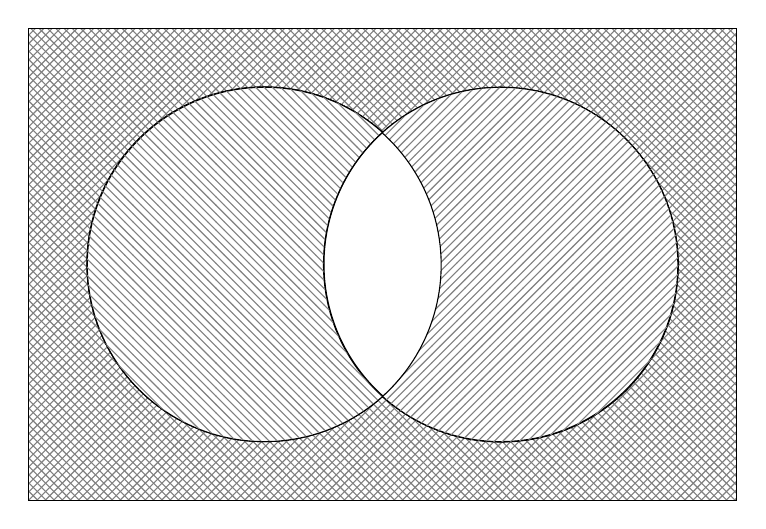
\begin{tikzpicture}[scale=3.0]
  \draw[pattern=north west lines, pattern color=gray] (0,0) rectangle
  ( 3,2 ); \draw[pattern=north east lines, pattern color=gray] (0,0)
  rectangle ( 3,2 );

  \draw[color=black] (1,1) circle( .75 ); \draw[color=black] (2,1)
  circle( .75); \draw[color=black] (1.5,1.559) arc( 48:312:.75 ) --
  (1.5,.441) arc( 228:132:.75 );

  \draw[color=black] (1.5,.441) arc( -132:132:.75 ) -- (1.5,1.559)
  arc( 48:-48:.75 );

  \draw[fill=white] (1,1) circle( .75 ); \draw[fill=white] (2,1)
  circle( .75 );
  
  \fill[pattern=north west lines, pattern color=gray] (1.5,1.559) arc(
  48:312:.75 ) -- (1.5,.441) arc( 228:132:.75 ) --cycle;
  
  \fill[pattern=north east lines, pattern color=gray] (1.5,.441) arc(
  -132:132:.75 ) -- (1.5,1.559) arc( 48:-48:.75 ) --cycle;

  \draw[color=black] (1.5,.441) arc( -48:48:.75 ) -- (1.5,1.559) arc(
  132:228:.75 ) --cycle;
\end{tikzpicture}

\begin{theorem}
  \label{thr:2.23}
  A set E is open if and only if its complement is closed
\end{theorem}
\begin{proof}
  Suppose $\compl{ E }$ is closed. Choose $x\in E$. Then $x \notin E$,
  and $x$ is not a limit point of $\compl{ E }$.  So there is a
  neighborhood of $x$ that is contained completely in $E$. This makes
  $x$ an interior point of E, and E is open.

  Suppose $E$ is open. Let x be a limit point of $\compl{ E }$. Every
  neighborhood of x contains a point of $\compl{ E }$. This means that
  $x$ is not an interior point of E, and since E is open,
  $x \in \compl{ E }$. Thus we see that $\compl{ E }$ is closed
\end{proof}

This also implies that a set F is closed if and only if its complement
is open.

\begin{theorem}
  \label{thr:2.24}
  Properties of unions and intersections of open and closed sets:
  \begin{itemize}
  \item For any collection of open sets, The union of them is open
  \item For any collection of closed sets, the intersection is closed
  \item For any finite collection of open sets, the intersection is
    open
  \item For any finite collection of closed sets, the union is closed.
  \end{itemize}
\end{theorem}
\begin{proof}
  For any interior point of a set, it is also an interior point of a
  union of that set and another, so the union of open sets must be
  open. Using the complements one can show that the intersection of
  closed sets is closed by the above two theorems.

  To see that the intersection of an infinite number of open sets
  doesn't have to be open, consider sets of intervals that are all
  subsets of each other, the intersection will be a single point, and
  therefore not be open.
\end{proof}

If X is a metric space, and $E \subset X$, The \emph{closure} of E is
the union of E and all of its limit points. It is denoted $\bar{E}$.

\begin{theorem}
  % Closure Properties
  \label{thr:2.27}
  For a metric space $X$ and $E \subset X$
  \begin{enumerate}
  \item $\close{E}$ is closed
  \item $E = \close{E}$ if and only if $E$ is closed
  \item $\close{E} \subset F$ for every closed set $F$ where:
    $E \subset F$
  \end{enumerate}
\end{theorem}
\begin{proof}
  \begin{enumerate}
  \item Any point in $\compl{ \bar{E} }$ has a neighborhood that does
    not intersect $E$, and therefore $\compl{ \bar{E} }$ is open. This
    implies $E$ is closed.
  \item If E is closed, then the limit points of E is a subset of E,
    and $E = \bar{E}$.
  \item If F is closed, than it contains its limit points, and
    therefore the limit points of E. So F is a super-set of the limit
    points of E as well as E, so it must be a super-set of the closure
    of E.
  \end{enumerate}
\end{proof}

This is effectively stating that the closure of a set is the
"smallest" closed set that contains the elements of the set.


\begin{theorem}
  \label{thr:2.28}
  Let E be a nonempty set of real numbers that is bounded above.  The
  supremum of this set is contained in the closure.
\end{theorem}
\begin{proof}
  Let $y=\sup{E}$. If $y \in E$ trivially true.

  For every $h > 0$, there is some $x \in E$ such that $y-h < x <y$ or
  $y-h$ would be a lower bound, and y couldn't be the least upper
  bound.

  This is exactly a neighborhood of y, and we have shown that it
  contains an element of E. This makes y a limit point of E, and thus
  $y \in \bar{E}$.
\end{proof}

When we speak of subsets, open and closed are conditions that are
relative to the super-set. As an interval can be open or not,
depending on whether or not it is a subset of $\setR$ or
$\setR^{k}$. To be clear on what the super-set is, we say \emph{open
  relative to} a set.

\begin{theorem}
  \label{thr:2.30}
  Suppose $Y\subset X$. A subset E of Y is open relative to Y if and
  only if $E = Y \cap G$ for some open subset G of X.
\end{theorem}

For the interval example, $E = (a,b), Y = \setR$ G is an open ball
around the midpoint of $(a,b)$ with diameter $b-a$.

\subsection{Compact Sets}
\label{sec:orgd64ebef}

An \emph{open cover} of a set E in some metric space $X$ is a
collection of open subsets of $X$ such that:
\begin{equation*}
  E \subset \bigcup_{\alpha} G_{\alpha}
\end{equation*}
Basically, the union of the sets "covers" the set E.

A subset K of a metric space $X$ is said to be \emph{compact} if every
open cover of K contains a finite sub-cover. This means that we could
cover K using only a finite number of sets.

Clearly, every finite set is compact, and there are a large number of
infinite compact sets. Compactness also does not rely on the
super-set. This means we do not need to consider the embedding space.

\begin{theorem}
  \label{thr:3.33}
  Suppose $K \subset Y \subset X$. Then K is compact relative to $X$
  if and only if K is compact relative to $Y$.
\end{theorem}
\begin{proof}
  Let K be compact relative to $X$. Let $\seq{V_{\alpha}}$ be a
  collection of sets that are open relative to Y and cover K.

  Since V is open relative to Y, each V can be written as:
  $V_{\alpha} = Y \cap G_{\alpha}$.\par
  These sets G form a cover for K, and as K is compact relative to X,
  $K \subset G_{\alpha_1} \cup ... \cup G_{\alpha_n}$.\par
  However since also: $K \subset Y$. We know that
  $K \subset V_{\alpha_1} \cup ... \cup V_{\alpha_n}$. Thus K is
  compact relative to Y. \par
  Let K be compact relative to Y, and let $\seq{G_{\alpha}} \subset X$
  be a cover of K. Let $V_{\alpha} = Y \cap G_{\alpha}$. $V_{\alpha}$
  forms a cover of K, and since K is compact in Y, there is a finite
  sub-cover of K. Since each G is a super-set of V, the particular Gs
  form a finite sub-cover of K in X as well.
\end{proof}

\begin{theorem}
  \label{thr:2.34}
  Compact subsets of metric spaces are closed
\end{theorem}
\begin{proof}
  Let K be a compact subset of a metric space X. We wish to show that
  its complement is open. \par
  Let $p \in \compl{ K }$. Consider a point $q \in K$. Take
  neighborhoods $V_q, W_q$ around $p$ and $q$ with radius less than
  $\met{p,q}$. \par
  Since K is compact, we need a finite number of q to cover K. If we
  take the intersection of all the neighborhoods of p, we have a
  neighborhood of p that does not intersect any $W_q$.

  This makes p and interior point of $K^c$ and thus K is closed.
\end{proof}

\begin{theorem}
  \label{thr:2.35}
  Closed subsets of compact sets are compact
\end{theorem}
\begin{proof}
  Honestly I couldn't understand this proof. It relies on the
  relationship between the compliment of a set and its cover.
\end{proof}

What this theorem does tell us though, is that if we have a closed set
and a compact set, then the intersection of the two is compact. As the
intersection between a closed and compact set is closed.

\begin{theorem}
  \label{thr:2.36}
  If $\seq{K_{\alpha}}$ is a collection of compact subsets of a metric
  space, where the intersection of every finite sub-collection is
  nonempty, then $\cap K_{\alpha}$ is nonempty.
\end{theorem}
\begin{proof}
  Assume that No point of $K_1$ belongs to $\cap K_{\alpha}$, Then all
  of $K_1$ is covered by the complement of the intersections. However
  since $K_1$ is compact, then there is a finite sub-cover of the
  complement that covers it, but this implies that the intersection
  over a finite number of the subsets is empty, which is a
  contradiction.
\end{proof}

This means that if we have a sequence of nonempty compact sets where
each successive one is a subset, then the infinite intersection is
nonempty.

\begin{theorem}
  \label{thr:2.37}
  If E is an infinite subset of a compact set K, then E has a limit
  point in K
\end{theorem}
\begin{proof}
  If this were not true, then every point $q \in K$ would have a
  neighborhood that contains at most one point of E ( q if $q \in E$.)
  This means no finite sub-collection of these neighborhoods can cover
  E, as E is infinite. This must be true of K, as it is a super-set of
  E. This is a contradiction.
\end{proof}

\begin{theorem}
  \label{thr:2.38}
  If $\seq{I_n}$ is a sequence of intervals in $\setR$ such that
  $I_n \supset I_{n+1}$ then $\cap_1^{\infty} I_n$ is not empty.
\end{theorem}
\begin{proof}
  For each interval $I_n = [a_n, b_n]$, Let $E$ be the smallest point
  in all the intervals.  E is nonempty and bounded above by $b_1$. Let
  $x = \sup{E}$. Since each interval is nested we know that
  $x \leq b_m \quad \forall m$. Then $x \in I_m \quad \forall m$.
\end{proof}

In fact this result extends to all k-cells

\begin{theorem}
  \label{thr:2.39}
  Let k be a positive integer, if $\seq{I_n}$ is a sequence of k-cells
  such that $I_n \supset I_{n+1}$ then $\cap_1^{\infty} I_n$ is not
  empty.
\end{theorem}
\begin{proof}
  Form a matrix of intervals, where the rows are each n, and the
  columns are the dimensions of the k-cells. Then we can simply follow
  the above theorem for each column, and choose the vector
  $x^* = ( x_1^*, ..., x_k^* )$
\end{proof}

\begin{theorem}
  \label{thr:2.40}
  Every k-cell is compact
\end{theorem}
\begin{proof}
  Let I be a k-cell, consistent of all points $\vec{x}$ such that
  $a_j \leq x_j \leq b_j$ Let
  $\delta = \brak{\sum_{j=1}^k ( b_j - a_j )^2}^{\frac{1}{2}}$ Then
  $\abs{\vec{x} - \vec{y}} \leq \delta$.

  Suppose that I is not compact, and let $c_j = \frac{a_j + b_j}{2}$
  The intervals $[a_j,c_j]$ and $[c_j,b_j]$ then determine $2^k$
  k-cells $Q_i$ whose union is I. Since I is not compact, at least one
  of these cells is not covered by any finite sub-collection of an
  open cover $G_{\alpha}$. Let this cell be denoted $I_1$. Continue
  this process on infinitely.

  This gives us a sequence $\seq{I_n}$ which has the following
  properties
  \begin{enumerate}
  \item $I \supset I_1 \supset I_2 \supset .... \supset I_n$
  \item $I_n$ is not covered by any finite sub-collection of
    $\seq{G_{\alpha}}$
  \item If $\vec{x} \in I_n$ and $\vec{y} \in I_n$ then
    $\abs{ \vec{x} - \vec{y}} \leq 2^{-n} \delta$
  \end{enumerate}
  From (1) we know that there is a point $\vec{x}$ which lies in every
  $I_n$. For some $\alpha$, $\vec{x}^{*} \in G_{\alpha}$ as G is a
  cover for I. Since $G_{\alpha}$ is open, there exists $r > 0$ such
  that $\abs{\vec{y} - \vec{x}^{*}} < r$ implies that
  $\vec{y} \in G_{\alpha}$.  Choose n to be large enough that
  $2^{-n}\delta < r$. This is possible from the Archimedian
  property. This means that (3) implies that $I_n \subset G_{\alpha}$
  which is contradicting (2).
\end{proof}

\begin{theorem}
  \label{thr:2.41}
  If a set E in $\setR^k$ has one of the following properties, then it
  has the rest:
  \begin{enumerate}
  \item E is closed and bounded
  \item E is compact
  \item Every infinite subset of E has a limit point in E
  \end{enumerate}
\end{theorem}
\begin{proof}
  If (1) holds, then $E \subset I$ for some k-cell I, and (2) follows
  immediately. We have shown already that (2) implies (3) so we only
  have to show that (3) implies (1).

  If E is not bounded, then E contains points $\vec{x}_n$ with
  $\abs{\vec{x}_n} > n$. The set S consisting of these points is
  infinite and has no limit points in $\setR^k$, and therefore none in
  E. Thus E must be bounded.

  If E is not closed, then there is a point $x_0 \in \setR^k$ which is
  a limit point of E but not a point of E. There are points
  $x_n \in E$ such that $\abs{x_n - x_0} < \frac{1}{n}$. Let S be the
  set of all of these points. Then S is infinite by the Archimedian
  property. S has $x_0$ as a limit point, and no other limit
  point. For some $\vec{y} \in \setR^k, \vec{y} \neq \vec{x}$.
  $\abs{x_n - \vec{y}} \geq \abs{x_0 - \vec{y}} - \abs{x_n - x_0} \geq
  |x_0 - \vec{y} - \frac{1}{n} \geq \frac{1}{2} \abs{ x_0 -
    \vec{y}}$. This means that $\vec{y}$ is not a limit point of S,
  and S has no limit point in E, so E must be closed for (3) to hold.
\end{proof}

In every metric space, (2) and (3) are equivalent, but (a) is only
equivalent to the other two in Borel spaces.

\begin{theorem}[Weierstrass]
  \label{thr:2.42}
  Every bounded infinite subset of $\setR^k$ has a limit point in
  $\setR^k$.
\end{theorem}
\begin{proof}
  Since the set is bounded, it is a subset of a k-cell I which is
  compact, and therefore the set has a limit point in I, which is in
  $\setR^k$.
\end{proof}

\subsubsection{Perfect Sets}
\label{sec:org48b86f9}

\begin{theorem}
  \label{thr:2.43}
  Let P be a nonempty perfect set in $\setR^k$. P is uncountable
\end{theorem}
\begin{proof}
  Since P has limit points, P must be infinite. Suppose P is countable
  and denote the points by $\seq{x}$. Then do some nonsense where you
  assume that the closure of neighborhoods have some properties and
  use the intersection with the closure and P to get compact sets that
  are empty, contradicting the fact they need to be nonempty.
\end{proof}

This is useful to showing that $[a,b]$ is uncountable for $(a<b)$. In
particular this means that the set of all Real numbers is uncountable.

\vspace{ .33in }

The cantor set: An uncountable perfect set that contains no segment
and has measure 0.

Form it the traditional way, removing the middle third of every
interval, and splitting each one in half.

\subsubsection{Connected Sets}
\label{sec:org9d40335}
Two subsets $A$ and $B$ of a metric space $X$ are said to be
\emph{separated} if both $A \cap \bar{B}$ and $\bar{A} \cap B$ are
empty. This means no point of A is in the closure of B and no point of
B is in the closure of A.

A set $E \subset X$ is said to be \emph{connected} if E is not a union of
two nonempty separated sets.

Separated is a stronger condition than disjoint, for example $[0,1]$
and $(1,2)$ are disjoint but not separated, as $1$ is a limit point of
$(1,2)$.

\begin{theorem}
  \label{thr:2.47}
  A subset E of a the real line $\setR$ is connected if and only if it
  has the following property: If
  $x \in E, y\in E, x < z < y \implies z \in E$
\end{theorem}
\begin{proof}
  If this were false, then there exists $x \in E, y \in E$ and some
  $z \in (x,y)$ such that $z \notin E$. Then $E = A_z \cup B_z$ where
  $A_z = E \cap (-\infty,z) B_z = E \cap (z,\infty)$. Since
  $x \in A_z$, $y \in B_z$ they must not be empty. They are clearly
  separated. Therefore E is not connected.
\end{proof}

\subsection{Exercises}
\label{sec:orgc8f61d7}
\subsubsection{Question 1}
\label{sec:orgb1ab764}
\begin{question}
  Prove that the empty set is a subset of every set
\end{question}
\begin{proof}
  For a set to be a subset, for all elements of the subset, they must
  be elements of the super-set. The empty set has no elements so this
  is vacuously true.
\end{proof}

\subsubsection{Question 2}
\label{sec:org6f8f04c}
\begin{question}
  Prove that the set of all algebraic numbers is countable

  Algebraic: There are integers $a_0, ..., a_n$ which are not all zero
  such that: $a_0 z^n + a_1 z^{n-1} + ... + a_{n-1}z + a_n = 0$.
  Hint: For every positive integer N, there are only finitely many
  equations with: $n + \abs{a_0} + \abs{a_1} + ... + \abs{a_n} = N$.
\end{question}
\begin{proof}
  Note that the set of all possible values for $a_i$ is
  countable. Therefore the set of all possible coefficients is an
  n-tuple of a countable set, and therefore countable. The set of
  coefficients for algebraic numbers is a subset of these numbers, and
  is at most countable. Clearly this set is not finite, as there are
  infinite degrees, and always at least one solution where
  $z=1, a_n = -\sum_{i=0}^{n-1}a_i$
 
  There is clearly an onto map from the coefficients to the algebraic
  numbers, this indicates that the cardinality of the algebraic
  numbers is less than or equal to the cardinality of the
  coefficients, and the algebraic numbers are at most countable.
  Assume that the algebraic numbers are finite. Since they are finite
  there must be a maximum, denote it $M$. Consider
  $M^{\prime} = \floor{M}+1$, Let $n=1, a_0 = -1, a_n =
  M^{\prime}$. Clearly $M^{\prime}$ must be an algebraic number,
  contradicting $M$ being the maximal element. Therefore the algebraic
  numbers are not finite, and therefore countable.


\end{proof}

\subsubsection{Question 4}
\label{sec:org1135e9c}
\begin{question}
  Is the set of all irrational real numbers countable?
\end{question}
\begin{proof}
  Denote the irrational numbers as: $\mathbb{I}$. Note that:
  $\setR = \mathbb{I} \cup \setQ$. Assume that $\mathbb{I}$ is
  countable. Then by theorem 2.12, The union of $\mathbb{I}$ and
  $\setQ$ must be countable, this however contradicts the fact that
  $\setR$ is not countable.
\end{proof}

\subsubsection{Question 5}
\label{sec:orgc85ac24}
\begin{question}
  Construct a bounded set of real numbers with exactly three limit
  points
\end{question}
\begin{proof}
  Consider a sequence of numbers $\seq{x}$ For each index k, using the
  division algorithm, generate numbers $r,w$ such that:
  $k = 3r + w, w \in \{0,1,2\}$. Let $x_k = \frac{1}{r} + 2w$ This
  clearly has 3 limit points: $\{0,2,4\}$.
\end{proof}

\subsubsection{Question 6}
\label{sec:org2dbd158}
\begin{question}
  Let $E^{\prime}$ be the set of all limit points of a set $E$. Prove
  that $E^{\prime}$ is closed.  Prove that $E$ and $\bar{E}$ have the
  same limit points. Do $E$ and $E^{\prime}$ always have the same
  limit points?
\end{question}
\begin{proof}
  \begin{enumerate}
  \item Assume that $E^{\prime}$ is not closed, let x be a limit point
    of $E^{\prime}$ that is not a limit point of $E$. Every
    neighborhood of x contains a limit point of E, and there is a
    number $\rho$ such that the neighborhood of radius $r \leq \rho$
    does not contain any point of E. Take $\epsilon =
    \frac{\rho}{3}$. For a neighborhood of radius $\epsilon$ there is
    a limit point contained in it, denote it y. Since y is a limit
    point of E, it contains a point in E within a neighborhood of
    radius $\epsilon$. Therefore the distance from that point in E to
    $x$ is at most $2\epsilon$ which is a contradiction to there being
    no points of E in a neighborhood of radius $r \leq \rho$.
  
  \item It is clear that there is no element of $E^{\prime}$ that is
    not contained in $\bar{E}$. All that remains to be shown is that
    there is no limit point of $\bar{E}$ that is not in
    $E^{\prime}$. Let $x$ be such a limit point. This means that every
    neighborhood of x contains a point of $E^{\prime}$ and some do not
    contain points of $E$. The same contradiction as above shows this
    is impossible.
    
  \item Yes by (1).
  \end{enumerate}
\end{proof}

\subsubsection{Question 8}
\label{sec:orgffec825}
\begin{question}
  Is every point of every open set $E \subset \setR^2$ a limit point
  of E?  Answer the same question for closed sets in $\setR^2$.
\end{question}
\begin{proof}
  Assume there is a point in an open set $E$ that is not a limit point
  of E. This means that it contains a neighborhood that is a subset of
  E, but not every neighborhood contains a point in E. This is
  impossible, as every smaller neighborhood remains a subset of E, and
  any larger neighborhood still contains at least one point from the
  neighborhood that is a subset of E.

  No, consider the set $[0,1] \cup \{ 2 \}$. Two is an isolated point
  of the set, and is not a limit point. More generally, any closed set
  that is not perfect will not have every point be a limit point.
\end{proof}

\subsubsection{Question 10}
\label{sec:orgdc5dc29}
\begin{question}
  Let $X$ be an infinite set. For $p \in X, q \in X$ define:
  
\begin{align*}
  \met{p,q} = 
  \begin{cases}
    1 \quad (\text{ if } p \neq q )\\
    0 \quad (\text{ if } p = q )\\
  \end{cases}
\end{align*}
Prove that this is a metric. Which subsets of the result metric space
are open? Which are closed? Which are compact?
\end{question}
\begin{proof}
  The first two conditions are trivially true, the triangle inequality
  remains to be demonstrated. We will consider several cases:

  Case: $\met{p,q} = 0$. Then $\met{p,r} + \met{r,q} \geq 0$ and the
  result holds

  Case: $\met{p,q} = 1, \met{p,r} = 0$ or $\met{r,q} = 0$ Then
  $\met{p,r} + \met{r,q} = 1 \geq \met{p,q}$

  Case: $\met{p,q} = 1, \met{p,r} = 1, \met{r,q} = 1$ Then
  $\met{p,r} + \met{r,q} = 2 \geq \met{p,q}$

  Note that it is impossible for
  $\met{p,q} = 1, \met{p,r} + \met{r,q} = 0$.

  In this metric space, there are no limit points, as neighborhoods
  with radius less than 1 contain only the center. This means that all
  sets are closed. Every point is also an interior point, so all
  subsets are open as well. Since there are no limit points in this
  set, no infinite subset is compact. Finite sets are still compact.
\end{proof}

\subsubsection{Question 11}
\label{sec:org67749a4}
\begin{question}
  \begin{enumerate}
  \item $\met{x,y}^1 = (x-y)^2$
  \item $\met{x,y}^2 = \sqrt{ \abs{ x - y }}$
  \item $\met{x,y}^3 = \abs{ x^2 - y^2}$
  \item $\met{x,y}^4 = \abs{ x - 2y}$
  \item $\met{x,y}^5 = \frac{\abs{x-y}}{1 + \abs{x-y}}$
  \end{enumerate}
  Determine which of these is a metric space or not in $\setR$
\end{question}
\begin{proof}
  \begin{enumerate}
  \item Clearly the first two properties are satisfied. Now consider
    the triangle inequality:
    $(x-z)^2 = ( (x-y) - (z-y) )^2 = (x-y)^2 + (z-y)^2 - 2(x-y)(z-y)$
    Note that if $y \in (x,z), 2(x-y)(z-y) < 0$ and the third
    inequality does not hold.

  \item Clearly the first two properties are satisfied. Since it is
    known that $\abs{x-y}$ is a metric:
    $\abs{x-y} \leq \abs{x-z} + \abs{z-y}$. Thus:
    $\sqrt{\abs{x-y}} \leq \sqrt{\abs{x-z} + \abs{z-y}}$. Note:
    $\sqrt{x+y} \leq \sqrt{ x + 2\sqrt{x}\sqrt{y} + y} = \sqrt{
      (\sqrt{x} + \sqrt{y})^2} = \sqrt{x} + \sqrt{y}$. Thus:
    $\sqrt{\abs{x-y}} \leq \sqrt{\abs{x-z}} + \sqrt{\abs{z-y}}$.
    
  \item Consider the points $x=2,y=-2$. $\met{x,y}^3 = 0$ despite
    $x\neq y$. Clearly this is not a metric space.
      
  \item Trivially the first two properties are satisfied.
    $\abs{x-2y} = \abs{(x-2z) + (z - 2y) + z} \leq \abs{ (x-2z) + (z -
      2y) } \leq \abs{ x - 2z} + \abs{z-2y}$

  \item We can see that: $\met{x,x}^{5}$ = 0, and
    $\met{x,y}^5 = \met{y,x}^5$. Note that:
    $\met{x,y} = 1 - \frac{1}{1+\abs{x-y}}$. Clearly the third
    property holds as the fraction reverses the triangle inequality,
    and the negative keeps the inequality correct.
  \end{enumerate}
\end{proof}
\subsubsection{Question 14}
\label{sec:org36afe95}
\begin{question}
  Give an example of an open cover of the segment $(0,1)$ which has no
  finite sub-cover
\end{question}
\begin{proof}
  Consider the sequence: $\seq{x}$ where $x_k = \frac{1}{k}$. Consider
  the sequence of segments: $\seq{s}$ where $s_k = (x_k, x_{k+1})$. By
  the Archimedian property this sequence is a cover of
  $(0,1)$. However any finite sub-cover of it must not contain every
  element of $(0,1)$ by the Archimedian property.
\end{proof}


\section{Numerical Sequences and Series}
\label{sec:3}

\subsection{Convergence Sequences}
\label{sec:3.1}
A sequence $\seq{p_{n}}$ in a metric space X is said to
\emph{converge} if there is a point $p \in X$ with the following
property:

For every $\epsilon > 0$ there is an integer N such that $n \geq N$
implies that $\met{ p_{n, }p} < \epsilon$.

In this case we also say that $\seq{p_{n}}$ converges to $p$ or that
$p$ is the limit of $\seq{p_{n}}$. We write: $p_{n} \to p$ or
$\Lim_{n \to \infty} p_{n} = p$

If $\seq{p_{n}}$ does not converge, it is said to \emph{diverge}.

It is useful to note that the notion of convergence relies upon the
metric space that we have embedded ourselves in. When it is ambiguous,
it will be specified \emph{convergent in $X$}.

The range of a sequence is the set of all the different points
$p_{n}$. It may be finite or infinite, and we say $\seq{p_{n}}$ is
bounded if its range is bounded.



\begin{theorem}
  \label{thr:3.2}
  Let $\seq{p_n}$ be a sequence in a metric space $X$.
  
  \begin{enumerate}
  \item $\seq{p_n}$ converges to $p \in X$ if and only if every
    neighborhood of $p$ contains $p_n$ for all but finitely many n
  \item If $p \in X, p^{\prime} \in X$, and if $\seq{p_n}$ converges
    to $p$ and $p^{\prime}$, then $p = p^{\prime}$.
  \item If $\seq{p_n}$ converges, then $\seq{p_n}$ is bounded.
  \item If $E \subset X$ and if $p$ is a limit point of $E$, then
    there is a sequence $\seq{p_n}$ in $E$ such that
    $p = \lim_{n \to \infty} p_n$.
  \end{enumerate}
\end{theorem}
\begin{proof}
  \begin{enumerate}
  \item Let $p_n \to p$ and let $V$ be a neighborhood of p.

    For some $\epsilon>0$, the conditions $\met{q,p} < \epsilon$ imply
    $q\in V$. Since $\seq{p_n}$ is convergent, there exists N such
    that $n \geq N \implies \met{p_n,p} < \epsilon$.

    Thus $n \geq N \implies p_n \in V$.  Conversely, if every
    neighborhood of p contains all but finitely many of the $p_n$.

    Fix $\epsilon > 0$ and let V be the set of all $q \in X$ such that
    $\met{p,q} < \epsilon$. Since all but finitely many lie in the
    neighborhood, there exists N (related to V) such that $p_n \in V$
    if $n \geq N$. Thus $\met{p_n,p}< \epsilon$ and $p_n \to p$.
  
  \item Let $\epsilon > 0$ be given. There exists integers $N, N'$
    such that:
    \begin{align*}
      n \geq N &\implies \met{ p_n, p} < \frac{\epsilon}{2}\\
      n \geq N' &\implies \met{ p_n, p'} < \frac{\epsilon}{2}\\
    \end{align*}
    Hence for all $n \geq \max \{ N, N' \}$ we get:
    $\met{p,p'} \leq \met{ p, p_n } + \met{ p_n, p'} < \epsilon$.
  
  \item Suppose $p_n \to p$. There is an integer N such that for
    $n > N, \met{p_n, p} < 1$. Let
    $r = \max\{ 1, \met{ p_1, p}, ..., \met{ p_N, p}\}$ Then
    $\met{p_n,p} \leq r \quad \forall n$.
  
  \item For each positive integer n, there is a point $p_n \in E$ such
    that $\met{p_n,p} < \frac{1}{n}$. For any $\epsilon > 0$ Choose
    $N = \floor{\frac{1}{\epsilon}}+1$ For all
    $n > N, \met{ p_n, p} < \epsilon$ and therefore $p_n \to p$
  \end{enumerate}
\end{proof}

For sequences in $\setR^{k}$ we can study the relation between
convergence and algebraic operations.

\begin{theorem}
  \label{thr:3.3}
  Suppose $\seq{s_n}, \seq{t_n}$ are complex sequences, and
  $\Lim_{n\to\infty}s_n = s, \Lim_{n\to\infty} t_n = t$ Then:
  \begin{enumerate}
  \item $\Lim_{n\to\infty} \left( s_n + t_n \right) = s + t$
  \item $\Lim_{n\to \infty} c s_n = cs$
  \item $\Lim_{n\to \infty} s_n t_n = st$
  \item $\Lim_{n \to \infty}\frac{1}{s_n} = \frac{1}{s}$ Provided:
    $s_n \neq 0, s \neq 0$.
  \end{enumerate}
\end{theorem}
\begin{proof}
  \begin{enumerate}
  \item For some $\epsilon > 0$, there exists integers $N_1, N_2$ such
    that: $n \geq N_1 \implies \abs{ s_n - s} < \frac{\epsilon}{2}$
    and $n \geq N_2 \implies \abs{ t_n - t} < \frac{\epsilon}{2}$.
    Choose $N = \max\{ N_1, N_2 \}$ then $n \geq N$ implies:
    $\abs{ s_n + t_n - s - t} \leq \abs{ s_n - s} + \abs{ t_n - t} <
    \epsilon$.
  
  \item Trivial as $c$ can be pulled out of $\abs{c s_n - cs}$
  \item $s_nt_n - st = (s_n -s )(t_n - t) + s( t_n - t) + t(s_n - s)$
    For some $\epsilon>0$ Do the same $N_1, N_2$ for
    $\sqrt{\epsilon}$. Let $N = \max\{ N_1, N_2 \}$ so that:
    $n \geq N \implies \abs{ (s_n-s)(t_n-t)} < \epsilon$ and:
    $\lim_{n\to \infty}(s_n-s)(t_n-t) = 0$. Applying this, as well as
    the convergence of $\seq{s_n} and \seq{t_n}$ to the original
    identity yields: $\lim_{n \to \infty} (s_n t_n - st ) = 0$.
  \item Choose $m$ such that $\abs{s_n-s} < \frac{1}{2} \abs{s}$ if
    $n \geq m$ Then $\abs{s_n} > \frac{1}{2}\abs{s}$ for $n \geq
    m$. For some $\epsilon > 0$ by convergence, there is an integer
    $N > m$ such that
    $n \geq N \implies \abs{s_n - s} < \frac{1}{2}\abs{s}^2
    \epsilon$. Thus:
    $\abs{ \frac{1}{s_n} - \frac{1}{s}} = \abs{\frac{s_n-s}{s_n s}} <
    \frac{2}{\abs{s}^2} \abs{ s_n - s} < \epsilon$
  \end{enumerate}
\end{proof}
That last proof made no sense to me either.

\begin{theorem}
  \label{thr:3.4}
  Suppose $\seq{\vec{x}_n} \in \setR^k$ and
  $\vec{x}_n = ( \alpha_{1,n}, ... \alpha_{k,n} )$. Then
  $\seq{\vec{x}_n}$ converges to
  $\vec{x} = ( \alpha_1, ..., \alpha_k )$ if and only if
  $\lim_{n\to \infty} \alpha_{j,n} = \alpha_j$.
\end{theorem}
\begin{proof}
  Let $\vec{x}_n \to \vec{x}$, Then from the definition of the norm in
  $\setR^k$ we get that:
  $\abs{ \alpha_{j,n}- \alpha_j} \leq \abs{\vec{x}_n - \vec{x}}$.

  Now let $\lim_{n\to \infty} \alpha_{j,n} = \alpha_j$. Then there is
  an integer N such that
  \begin{align*}
    n \geq N &\implies \abs{ \alpha_{j,n} - \alpha_j} <
               \frac{\epsilon}{\sqrt{k}}\\
    n \geq N &\implies \abs{ \vec{x}_n - \vec{x}} = \brak{
               \sum_{j=1}^k \abs{ \alpha_{j,n} - \alpha_j}^2 }^{\frac{1}{2}} < \epsilon
  \end{align*}
  This implies that $\vec{x}_n \to \vec{x}$.
\end{proof}

All the properties of sums, dot products and scalar products in
convergence hold for sequences of vectors as well.

\subsection{Subsequences}
\label{sec:3.2}
For some sequence $\seq{p_{n}}$, consider a sequence $\seq{n_{k}}$ of
strictly increasing positive integers. Then the sequence
$\seq{p_{n_{i}}}$ is called a \emph{subsequence} of $\seq{p_{n}}$. If
$\seq{p_{n_{i}}}$ converges, its limit is called a \emph{subsequential
  limit} of $\seq{p_{n}}$.

\begin{theorem}
  % Not proved in the book
  \label{thr:3.0}
  A sequence $\seq{p_n}$ converges to $p$ if and only if every
  subsequence of $\seq{p_n}$ converges to $p$.
\end{theorem}
\begin{proof}
  Consider a convergent sequence $\seq{p_n}$, For some $\epsilon > 0$
  and some arbitrary subsequence, choose
  $N_k = \min \{n_i, n_i \geq N \}$. It is clear that for all
  $n \geq N_k, \abs{ p_{n_i} - p} < \epsilon$.

  For the converse, assume that every subsequence is convergent to
  p. For some $\epsilon > 0$ Take $N = \max \{ N_i \}$. Clearly for
  all $n \geq N, \abs{ p_n - p} < \epsilon$.
\end{proof}

\begin{theorem}
  \label{thr:3.6}
  \begin{enumerate}
  \item If $\seq{p_n}$ is a sequence in a compact metric space X, then
    some subsequence of $\seq{p_n}$ converges to a point of X
  \item Every bounded sequence in $\setR^k$ contains a convergent
    subsequence.
  \end{enumerate}
\end{theorem}
\begin{proof}
  \begin{enumerate}
  \item Let E be the range of $\seq{p_n}$. If E is finite, then there
    is a sequence of indices such that
    $p_{n_1} = p_{n_2} = ... = p_{n_k} = p$. Clearly it converges.

    If E is infinite, theorem \ref{thr:2.37} indicates that E has a
    limit point $p \in X$. Since it has a limit point, every
    neighborhood contains an element of $\seq{p_n}$ Choose each $n_i$
    such that $p_{n_i}$ lies in a neighborhood with radius
    $\frac{1}{i}$. This subsequence must converge to p.
  \item Since every bounded subset of $\setR^k$ lies in a compact
    subset of $\setR^k$ this result follows immediately from part (1).
  \end{enumerate}
\end{proof}

\begin{theorem}
  \label{thr:3.7}
  The sub-sequential limits of a sequence $\seq{p_n}$ in a metric
  space $X$ form a closed subset of $X$.
\end{theorem}
\begin{proof}
  Let $E^{*}$ be the set of all sub-sequential limits of $\seq{p_n}$
  and let $q$ be a limit point of $E^{*}$. We wish to show that
  $q \in E^{*}$.

  Choose $n_1$ so that $p_{n_1} \neq q$. If this is not possible, then
  the sequence has only one point and we are done. Let
  $\delta = \met{ q, p_{n_1}}$. Since $q$ is a limit point of $E^{*}$,
  we can choose $n_i$ such that $\met{q,p_{n_i}} < 2^{-i}\delta$. We
  can see that this sequence will converge to $q$ and $q \in E^{*}$.
\end{proof}

\subsection{Cauchy Sequences}
\label{sec:org6bbcfd8}

A sequence $\seq{p_n}$ in a metric space $X$ is said to be a
\emph{Cauchy sequence} if for every $\epsilon >0$ there is an integer
N such that $\met{p_n, p_m} < \epsilon$ if $n \geq N$ and $m \geq N$.

Let $E$ be a nonempty subset of a metric space $X$, the
\emph{diameter} of a set is the supremum of $\met{p,q}$ over all
$p \in E, q \in E$.

For a sequence $\seq{p_{n}} \in X$. Let $E_N$ be the range of
$\seq{p_n}$. It is clear that $\seq{p_n}$ is a Cauchy sequence if and
only if: $\lim_{N\to\infty} \diam{ E_N } = 0$

\begin{theorem}
  \label{thr:3.10}
  \begin{enumerate}
  \item If $\close{E}$ is the closure of a set $E$ in a metric space
    X, then $\diam{\close{E}} = \diam{E}$
  \item If $\seq{K_n}$ is a sequence of compact sets in X such that
    $K_n \supset K_{n+1}$ and $\lim_{n\to \infty} \diam{K_n} = 0$ Then
    $\cap_1^{\infty} K_n$ consists of exactly one point.
  \end{enumerate}
\end{theorem}
\begin{proof}
  \begin{enumerate}
  \item Since $E \subset \close{E}$, it is clear that:
    $\diam{E} \leq \diam{\close{E}}$. Fix $\epsilon > 0$ and choose
    $p \in \close{E}, q \in \close{E}$. By the definition of
    $\close{E}$, there are points $p', q'$ in $E$ such that
    $\met{p, p'} < \epsilon, \met{q,q'} < \epsilon$. Hence:
    \begin{align*}
      \met{p,q} &\leq \met{ p, p'} + \met{ p', q'} + \met{ q', q}\\
                &< 2\epsilon + \met{ p', q'} \leq 2\epsilon + \diam{E}\\
    \end{align*}

    Since $\diam{\close{E}}$ is the supremum over all $p,q$, and we
    know that $\close{E}$ is closed, we may choose $p,q$ such that
    $\met{p,q} = \diam{\close{E}}$. Then:
    $\diam{\close{E}} \leq 2\epsilon + \diam{E}$ and since $\epsilon$
    was arbitrary, we have $\diam{E} = \diam{\close{E}}$.
  \item Let $K = \cap_1^{\infty} K_n$, it is known that $K$ is not
    empty. If $K$ contains more than one point, $\diam{K} > 0$. But we
    know that since $K \subset K_n, \diam{K} \leq \diam{K_n}$ This
    contradicts $\diam{K_n} \to 0$ So $K$ must contain only one point.
  \end{enumerate}
\end{proof}

\begin{theorem}
  \label{thr:3.11}
  \begin{enumerate}
  \item In any metric space $X$, every convergent sequence is a Cauchy
    sequence
  \item If $X$ is a compact metric space and if $\seq{p_n}$ is a
    Cauchy sequence in $X$, then $\seq{p_n}$ converges to some point
    of X.
  \item In $\setR^k$, every Cauchy sequence converges
  \end{enumerate}
\end{theorem}
\begin{proof}
  \begin{enumerate}
  \item If $p_n \to p$ and if $\epsilon > 0$, there is an integer $N$
    such that $\met{p,p_n} < \epsilon$ for all $n \geq N$.  Hence:
    $\met{p_n, p_m} \leq \met{ p_n, p} + \met{ p, p_m} < 2\epsilon$ if
    $n \geq N, m \geq N$. This means that $\seq{p_n}$ is a Cauchy
    sequence.
  \item Let $\seq{p_n}$ be a Cauchy sequence in the compact space $X$.
    For $N \in \setN$, let $E_N$ be the set consisting of
    $p_N, p_{N+1}, ...$ Then:
    $\lim_{N \to \infty} \diam{ \close{E_N}} = 0$. Since $\close{E_N}$
    is a closed subset of a compact space, they are all compact.  and
    $\close{E_N} \supset \close{E_{N+1}}$.  Their infinite
    intersection therefore contains only one point by the above
    theorem. Call this point $p \in \close{E_N}$. Since the limit of
    the diameter tends to zero, and $p$ is in the sequence,
    $\seq{p_n} \to p$.
  \item Let $\seq{\vec{x}_n}$ be a Cauchy sequence in
    $\setR^k$. Define $E_N$ the same as above. For some N,
    $\diam{E_N} < 1$. The range of $\seq{\vec{x}_n}$ is the union of
    $E_N$ and the finite set of the previous values of
    $\seq{\vec{x}_n}$. This means that $\seq{\vec{x}_n}$ is
    bounded. Every bounded subset of $\setR^k$ has compact closure in
    $\setR^k$, this result follows from above.
  \end{enumerate}
\end{proof}

A metric space in which every Cauchy sequence converges is said to be
\emph{complete}.

The above theorem can be extended to now say: all compact metric
spaces are complete, as well as all Euclidean spaces. It also implies
that every closed subset of a complete metric space is complete.

\subsection{Monotonic Sequences}
\label{sec:org803e73d}

A sequence $\seq{s_n}$ of real numbers is said to be
\begin{itemize}
\item \emph{monotonically increasing} if $s_n \leq s_{n+1}$
\item \emph{monotonically decreasing} if $s_n \geq s_{n+1}$
\end{itemize}

The class of monotonic sequences consists of the increasing and
decreasing sequences.

\begin{theorem}
  \label{thr:3.14}
  Suppose $\seq{s_n}$ is monotonic. Then $\seq{s_n}$ converges if and
  only if it is bounded.
\end{theorem}
\begin{proof}
  Let $\seq{s_n}$ be a monotonically increasing sequence. Let $E$ be
  the range. Assume $\seq{s_n}$ is bounded, and let $s$ be the least
  upper bound of $E$. It is clear that $s_n \leq s$ and for every
  $\epsilon > 0$ there is an integer N such that:
  $s - \epsilon < s_N \leq s$. This happens because $s$ is the least
  upper bound. This is convergence to $s$.

  The converse has already been established, as all convergent
  sequences are bounded.
\end{proof}

\subsection{Upper and Lower Limits}
\label{sec:orgcc73cf4}
Let $\seq{s_n}$ be a sequence of real numbers. Let $E$ be the set of
subsequential limits and $\set{\infty, -\infty}$ for divergent
subsequences. Let $s^{*} = \sup{E}$ and $s_{*} = \inf{E}$. These
numbers are called the \emph{upper} and \emph{lower} limits of
$\seq{s_n}$. The more common notation is:
\begin{equation*}
  \limsup_{n\to \infty} s_n = s^{*} \quad \liminf_{n\to \infty} s_n = s_{*}
\end{equation*}

\begin{theorem}
  \label{thr:3.17}
  Let $\seq{s_n}$ be a sequence of real numbers, Using the above
  definitions for $E$ and $s^{*}$. $s^{*}$ is the only number with the
  following two properties
  \begin{enumerate}
  \item $s^{*} \in E$
  \item If $x > s^{*}$, there is an integer $N$ such that $n \geq N$
    implies $s_n < x$
  \end{enumerate}
  The same is true in opposite for $s_{*}$.
\end{theorem}

\begin{proof}
  \begin{enumerate}
  \item If $s^{*} = \infty$, then E is not bounded above and
    $\seq{s_n}$ is not bounded above, so there is a subsequence that
    converges to $\infty$.

    If $s^{*}$ is real, then $E$ is bounded above and at least one
    subsequential limit exists, and the result comes from theorem
    \ref{thr:3.7}.

    If $s^{*} = -\infty$, then E contains only one element, so the
    result is trivial
  \item Suppose there is a number $x > s^{*}$ such that $s_n \geq x$
    for all values of n, that means there is a convergent subsequence
    that has a limit above $s^{*}$ which contradicts it being the
    supremum.
  \item uniqueness arises from the second property immediately driving
    uniqueness.
  \end{enumerate}
\end{proof}

\begin{theorem}
  % bounds of $\limsup$ and $\liminf$
  \label{thr:3.19}
  If $s_n \leq t_n$ for $n \geq N$ where N is fixed then:
  \begin{align*}
    \liminf_{n\to \infty}s_n &\leq \liminf_{n\to \infty}t_n\\
    \limsup_{n\to\infty}s_n &\leq \limsup_{n\to \infty}t_n\\
  \end{align*}
\end{theorem}

\subsection*{Special Sequences}

\begin{theorem}
  % special sequences
  \label{thr:3.20}
  \begin{enumerate}
  \item If $p > 0$ then $\Lim_{n\to\infty} \frac{1}{n^p} = 0$
  \item If $p > 0$ then $\Lim_{N\to\infty} p^{\frac{1}{p}} = 1$
  \item $\Lim_{n \to\infty} n^{\frac{1}{n}} = 1$
  \item IF $p > 0$ and $\alpha$ is real, then
    $\Lim_{N\to\infty} \frac{n^{\alpha}}{(1+p)^n} = 0$
  \item If $\abs{x} < 1$ then $\Lim_{n\to\infty} x^n = 0$
  \end{enumerate}
\end{theorem}
\begin{proof}
  \begin{enumerate}
  \item Take $n > \frac{1}{\epsilon}^{\frac{1}{p}}$ This is possible
    by the Archimedian property.
  \item If $p > 1$ put $x_n = p^{\frac{1}{n}} -1$ Then $x_n > 0$ and
    by the binomial theorem:
    \begin{align*}
      1 + nx_n &\leq (1+x_n)^n = p\\
      0 &< x_n \leq \frac{p-1}{n}\\
    \end{align*}
    Then: $x_n \to 0$. If $p = 1$ the result is trivial. If
    $p \in (0,1)$ simply take the reciprocal and repeat process for
    $p > 1$
  \item Put $X_n = n^{\frac{1}{n}} - 1$ Then $x_n \geq 0$ and from the
    binomial theorem:
    \begin{align*}
      n &= (1+x_n)^n \geq \frac{n(n-1)}{2} x_n^2\\
      0 &\leq x_n \leq \sqrt{ \frac{2}{n-1}} (n \geq 2 )\\
    \end{align*}
  \item Let $k$ be an integer such that $k > \alpha, k > 0$. For
    $n > 2k$
    \begin{align*}
      (1+p)^n > \binom{n}{k} p^k > \frac{n^kp^k}{2^kk!}\\
      0 < \frac{n^{\alpha}}{(1+p)^n} < \frac{2^k k!}{p^k} n^{\alpha-k} (n > 2k)
    \end{align*}
  \item Take $\alpha = 0$ in the above example.
  \end{enumerate}
\end{proof}

\subsection*{Series}

Series are omitted for the sake of time.

\subsection*{The Number e}

Let $e = \sum_{n=0}^{\infty} \frac{1}{n!}$ We can see that this series
converges because of:
\begin{align*}
  s_n &= 1 + 1 + \frac{1}{1 \cdot 2} + \frac{1}{1 \cdot 2 \cdot 3} + ... +
        \frac{1}{1 \cdot2 \cdot 3 \cdot .... \cdot n}\\
      &< 1 + 1 + \frac{1}{2} + \frac{1}{2^2} + ... + \frac{1}{2^{n-1}} < 3\\
\end{align*}

\begin{theorem}
  % definition of e
  \label{thr:31}
  $\Lim_{n\to\infty} \left ( 1 + \frac{1}{n} \right )^n = e$
\end{theorem}
\begin{proof}
  Let
  \begin{equation*}
    s_n = \sum_{k=0}^n \frac{1}{k!} \quad t_n = \brak{ 1 + \frac{1}{n}}^n
  \end{equation*}
  From the binomial theorem:
  \begin{equation*}
    t_n = 1 + 1 + \frac{1}{2!}( 1 - \frac{1}{n} ) + \frac{1}{3!}( 1 -
    \frac{1}{n} )( 1 - \frac{2}{n}) + ... + \frac{1}{n!}( 1 -
    \frac{1}{n})...(1 - \frac{n-1}{n})
  \end{equation*}
  Hence: $t_n \leq s_n$ so that: $\limsup_{n\to\infty}t_n \leq e$. by
  theorem \ref{thr:3.19}. Next if $n \geq m$
  \begin{equation*}
    tn \geq 1 + 1 + \frac{1}{2!}( 1 - \frac{1}{n} ) + ... +
    \frac{1}{m!}(1-\frac{1}{n})...(1 - \frac{m-1}{n} )
  \end{equation*}
  Letting $n \to \infty$ keeping $m$ fixed. We get
  \begin{equation*}
    \liminf_{n\to\infty}t_n \geq 1 + 1 + \frac{1}{2!} + ... + \frac{1}{m!}
  \end{equation*}
  so that: $s_m \leq \liminf_{n\to\infty} t_n$. Letting $m \to \infty$
  we finally get $e \leq \liminf_{n\to\infty} t_n$ and we see that the
  two sequences converge to the same limit.
\end{proof}

\begin{theorem}
  \label{thr:3.32}
  e is irrational
\end{theorem}
\begin{proof}
  Suppose e is rational, then $e = \frac{p}{q}$ where $p,q \in \setN$
  and irreducible. Using the inequality:
  $0 < e - s_n < \frac{1}{n!  n}$ we can plug in $n = q$ and arrive
  at:
  \begin{equation*}
    0 < q! ( e - s_q ) < \frac{1}{q}
  \end{equation*}
  By assumption: $q!e$ is an integer, and
  $q! s_q = q!( 1 + 1 + \frac{1}{2!} + ... + \frac{1}{q!} )$ which is
  an integer. Clearly: $q!  ( e - s_q)$ is an integer. \par
  However, we know that $q$ is an integer so: $q \geq 1$ and
  $ 0 < q!( e - s_q ) < 1$ which is a contradiction for an integer.
\end{proof}

In actuality, $e$ is not even an algebraic number. However a proof is
not supplied and can easily be googled.

\subsection*{Exercises}

\subsubsection*{Question 1}

\begin{question}
  Prove that convergence of $\seq{s_n}$ implies convergence of
  $\seq{\abs{s_n}}$. Is the converse true?
\end{question}
\begin{proof}
  Let $\seq{s_n}$ be a convergent sequence, then for $\epsilon > 0$
  and for all $n \geq N$ $\abs{ s_n - s} < \epsilon$. Note that:
  $\abs{ \abs{s_n} - \abs{s}} \leq \abs{s_n -s } < \epsilon$ so
  clearly $\abs{s_n}$ converges to: $\abs{s}$.

  The converse is not true, consider the sequence $s_k = (-1)^k$. This
  sequence is divergent, but its absolute value is a constant
  sequence.
\end{proof}

\subsubsection*{Question 2}

\begin{question}
  Calculate $\Lim_{n\to\infty} \sqrt{ n^2 + n} - n$
\end{question}
\begin{proof}
  \begin{align*}
    \sqrt{ n^2 + n} - n          &= \sqrt{ n^2 + n} - n \frac{\sqrt{ n^2 + n}
                                   +n}{\sqrt{n^2 + n} + n}\\
                                 &= \frac{n^2 + n - n^2}{\sqrt{ n^2 + n} + n}\\
    \text{only holds with n > 0} &= \frac{1}{\sqrt{1 + \frac{1}{n}} + 1}\\
    \Lim_{n\to \infty}\sqrt{ n^2 + n}- n &= \frac{1}{2}\\
  \end{align*}
\end{proof}

\subsubsection*{Question 3}

\begin{question}
  Let $s_1 = \sqrt{2}, s_{n+1} = \sqrt{ 2 + \sqrt{s_n}}$ Prove that
  $\seq{s_n}$ converges and that $s_n < 2$.
\end{question}
\begin{proof}
  Note that: $s_n$ is positive for all $n$, so it is equivalent to
  consider the convergence of $s_n^2$. $s_{n+1}^2 = 2 + \sqrt{s_n}$.

  We wish to show that this sequence is increasing and bounded above.

  Bounded above: Approach by induction. It is clear that $s_1 <
  2$. Assume that $s_n < 2$, $s_{n+1}^2 = 2 + \sqrt{s_n}$. From the
  inductive hypothesis we see that: $s_{n+1}^2 < 2 +\sqrt{2} < 4$ and
  $s_{n+1} < 2$. By induction we can see that $s_n$ is bounded above
  by 2.

  Increasing:
  \begin{align*}
    s_n - s_{n+1} &= s_n - \sqrt{ 2 + \sqrt{s_n}}\\
                  &\leq s_n - \sqrt{2} - s_n^{\frac{1}{4}}\\
                  &< s_n - \sqrt{2}\\
                  &< 0 \text{ for } s_n < 2\\    
  \end{align*}  
\end{proof}

\subsubsection*{Question 4}

\begin{question}
  Find the upper and lower limits of the sequence $\seq{s_n}$ defined
  by:
  \begin{equation*}
    s_1 = 0 \quad s_{2m} = \frac{s_{2m-1}}{2} \quad s_{2m+1} = \frac{1}{2} + s_{2m}
  \end{equation*}
\end{question}
\begin{proof}
  Clearly the lower limit of this sequence is zero, as neither
  operation can decrease the sequence.

  Consider the subsequence made of only the odd elements:
  $s_0 = 0, s_k = \frac{s_{k-1}+1}{2} = \frac{2^k-1}{2^k}$.

  The subsequence made of the even elements:
  $s_0 = 0, s_k = \frac{1+2s_{k-1}}{4} =
  \frac{2^{k+1}-2^k-1}{2^{k+1}}$

  Any other convergent subsequence must be subsequences of these
  subsequences. Their limits are clearly $1, \frac{1}{2}$. The
  supremum of this set then is $1$.
\end{proof}

\subsubsection*{Question 14}

\begin{question}
  If $\seq{s_n}$ is a complex sequence, its arithmetic mean is defined
  by:
  \begin{equation*}
    \sigma_n = \frac{s_0 + s_1 + ... + s_n}{n+1}
  \end{equation*}
  \begin{enumerate}
  \item If $\lim_{n\to\infty}s_n = s$ prove that
    $\Lim_{n\to\infty} \sigma_n = s$
  \item Construct a sequence $\seq{s_n}$ which does not converge
    although $\lim \sigma_n = 0$
  \item Can it happen that $s_n > 0$ and that $\limsup s_n = \infty$
    but $lim \sigma_n = 0$
  \item Put $a_n = s_n - s_{n-1}$. Show that:
    \begin{equation*}
      s_n - \sigma_n = \frac{1}{n+1} \sum_{k=1}^n k a_k
    \end{equation*}
    Assume that $\lim (n a_n) = 0$ and that $\seq{\sigma_n}$ converges
    to $\sigma$.
  \end{enumerate}
\end{question}
\begin{proof}
  \begin{enumerate}
  \item Note that since $\seq{s_n}$ is convergent, it is bounded. Call
    its upper bound $M$
    \begin{align*}
      \abs{\sigma_n -s } &= \abs{ \frac{s_0 + s_1 + ... + s_n }{n+1} -
                           \frac{s(n+1)}{n+1}}\\
                         &= \abs{ \frac{ (s_0 - s) + (s_1 - s) +
                           ... + (s_n - s)}{n+1}}\\
                         &\leq \frac{\abs{s_0 -s }}{n+1} +
                           \frac{\abs{s_1-s}}{n+1} + ... +
                           \frac{\abs{s_n-s}}{n+1}\\
                         &< \frac{NM}{n+1} + \frac{(n+1-N)\epsilon}{n+1}\\
    \end{align*}
    It is clear that the first term can be made arbitrarily small, and
    the second term always remains less than $\epsilon$. Clearly this
    sequence converges.
  \item Consider the sequence $\seq{s_n} = (-1)^n$. It is clearly
    divergent, however the limit of its arithmetic mean is 0.
  \item No, for the sum of a strictly positive sequence divided by a
    strictly positive number to converge to zero, the sequence must
    converge to zero.

    Assume otherwise. Claim there is a number M such that infinitely
    many of $s_n \geq M$. Then
    $s_0 + s_1 + ... + s_n \geq n \min\{ s_i \}$ for some $n > 0$. and
    when divided by n, this tends to the minimum, which is not zero.

    However if the sequence converges to zero, then no subsequence can
    be divergent, and it is impossible for $\limsup s_n = \infty$.
  \item
    \begin{align*}
      s_n - \sigma_n &= \frac{(n+1)s_n - s_0 - s_1 - ... - s_n}{n+1}\\
      \sum_{k=1}^n ka_k &= \sum_{k=1}^n k ( s_n - s_{n-1} )\\
                     &= \sum_{k=1}^n - s_k + n s_n \\
      s_n - \sigma_n &= \frac{1}{n+1} \sum_{k=1}^n k a_k\\
    \end{align*}
    We wish to show that:
    $\frac{1}{n+1} \sum_{k=1}^n \brak{ k a_k } + \sigma_n$ converges.
  \end{enumerate}
\end{proof}

\section{Limits and Continuity}

\subsection{Limits}

For metric spaces $X$ and $Y$, Let $E \subset Y$, $f$ maps $E$ into
$Y$ and $p$ be a limit point of $E$. We write: $f(x) \to q$ as
$x \to p$ or $\Lim_{x\to p}f(x) = q$ if there is a point $q \in Y$
with the following property:

For every $\epsilon > 0$ there exists a $\delta > 0$ such that:
$\met{ f(x), q } < \epsilon$ for all points $x \in E$ for which
$0 < \met{ x, p } < \delta$.

Note that although $p \in X$, $p$ does not need to be a point of $E$,
and even if $p$ is a point in $E$, the limit does not need to equal
the function at that point.

Since this definition is concerned with limit points, which can be
viewed as limits of sequences, there is an equivalent definition for a
limit using sequences:

We say that: $\Lim_{x\to p}f(x) = q$ if and only if
$\Lim_{n \to \infty} f( p_n ) = q$ for every sequence $\seq{p_n}$ in
$E$ such that: $p_n \neq p, \Lim_{n \to \infty}p_n = p$

\begin{proof}
  Let $f$ be a function such that: $\Lim_{x\to p} f(x) = q$, and let
  $\seq{p_n}$ be a sequence in $E$ such that
  $p_n \neq p, \Lim_{n\to \infty}p_n = p$. For some $\epsilon>0$,
  there exists $\delta > 0$ such that: $\met{f(x),q} < \epsilon$ if
  $x \in E$ and $0 < \met{x,p} < \delta$.

  For a the sequence $\seq{p_n}$, there exists some $N$ such that
  $n > N$ implies $0 < \met{p_n,p} < \delta$. So taking $x = p_n$,
  $\met{f(p_n), q} < \epsilon$ and shows that
  $Lim_{n\to\infty}f(p_n) = q$.

  Now suppose that $f$ does not have limit $q$ as $x \to p$. For some
  $\epsilon > 0$, for every $\delta > 0$ there is some point $x \in E$
  for which $\met{f(x),q} \geq \epsilon$, but
  $0 < \met{x,p} < \delta$.

  Let $p_n = p +/- \frac{1}{n}$, or its projection into E, then
  $p_n \neq p$ as p is a limit point, and $\Lim_{n\to \infty}p_n =
  p$. However, $\Lim_{n\to\infty} f( p_n ) \neq q$.
\end{proof}

Since limits of sequences have already been proved to be unique, this
definition tells us that if $f$ has a limit at $p$, then this limit is
unique.

\begin{theorem}
  \label{thr:4.4}
  Suppose $E \subset X$ is a metric space, $p$ is a limit point of $E$
  and $f,g$ are complex functions on $E$ such that:
  $\Lim_{x\to p} f(x) = A, \Lim_{x\to p}g(x) = B$. Then:
  \begin{enumerate}
  \item $\Lim_{x\to p}(f+g)(x) = A + B$
  \item $\Lim_{x\to p}(fg)(x) = AB$
  \item $\Lim_{x\to p}(\frac{f}{g})(x) = \frac{A}{B}$ for $B \neq 0$
  \end{enumerate}
\end{theorem}
These follow immediately form their proofs of the sequences.

If $f,g$ are mapping $E$ into $\setR^k$ then instead of multiplication
and division, the limit property of the scalar product remains true:
\newline $\Lim_{x\to p}(f \cdot g)(x) = A\cdot B$.


\subsection{Continuous functions}
Let $X$ and $Y$ be metric spaces, $E \subset X, p \in E$ and $f$ maps
$E$ into $Y$. Then $f$ is said to be \emph{continuous at $p$} if for
every $\epsilon > 0 $ there exists a $\delta > 0$ such that:
$\met{f(x),f(p)} < \epsilon$.

If $f$ is continuous at every point of $E$, then $f$ is said to be
\emph{continuous on $E$}.

Note that $f$ has to be defined at the point $p$ in order to be
continuous at $p$. However there is no requirement that $p$ is a limit
point, continuity is defined for isolated points as well. A function
is always continuous at isolated points, as there is a neighborhood
that contains no points of $E$ besides $p$.

\begin{theorem}
  \label{thr:4.6}
  When $p$ is a limit point of E, $f$ is continuous at $p$ if and only
  if $\Lim_{x \to p}f(x) = f(p)$.
\end{theorem}

\begin{theorem}
  \label{thr:4.7}
  Suppose $X,Y,Z$ are metric spaces, $E \subset X$, $f$ maps $E$ into
  $Y$, $g$ maps $f(E)$ into $Z$ and $h$ is the mapping of $E$ into $Z$
  defined by $h(x) = g(f(x))$

  If $f$ is continuous at a point $p \in E$ and if $g$ is continuous
  at the point $f(p)$ then $h$ is continuous at $p$.

  This function $h$ is called the \emph{composition} of $f$ and $g$
  and is denoted: $h = f \compose g$
\end{theorem}

\begin{proof}
  Let $\epsilon > 0$, since g is continuous at $f(p)$ there exists
  $\eta > 0$ such that: $\met{ g(y),g(f(p))} < \epsilon$ if
  $\met{y,f(p)} < \eta$ and $y \in f(E)$.

  Since $f$ is continuous at $p$, there exists $\delta > 0$ such that:
  $\met{f(x), f(p)} < \eta$ if $\met{x,p} < \delta$ and $x \in
  E$. Thus we can see that:
  $\met{h(x),h(p)} = \met{ g(f(x)), g(f(p)) } < \epsilon$ For
  $\met{x,p} < \delta$ and $x \in E$. Thus $h$ is continuous at $p$.
\end{proof}

\begin{theorem}
  \label{thr:4.8}
  A mapping $f$ of a metric space $X$ into a metric space $Y$ is
  continuous on $X$ if and only if $\inverse{f}(V)$ is open in $X$ for
  every open set $V$ in $Y$.
\end{theorem}

\begin{proof}
  Suppose $f$ is continuous on $X$ and $V$ is an open set in $Y$. We
  wish to show that every point of $\inverse{f}(V)$ is an interior
  point of $\inverse{f}(V)$.

  Suppose $p \in X$ and $f(p) \in V$. Since $V$ is open, there exists
  $\epsilon > 0$ such that $y \in V$ if $\met{y,p} < \epsilon$. Since
  $f$ is continuous at $p$, there exists $\delta > 0$ such that
  $\met{f(x), f(p)} < \epsilon$ if $\met{x,p} < \delta$. Thus:
  $x \in \inverse{f}(V)$ if $\met{x,p} < \delta$. This gives a
  neighborhood of $p$ that is a subset of $\inverse{f}(V)$ and thus it
  is open.

  Conversely: Suppose that $\inverse{f}(V)$ is open in $X$ for every
  open set $V$ in $Y$. Fix $p \in X, \epsilon > 0$ and let $V$ be the
  set of all $y \in Y$ such that $\met{y,f(p)} < \epsilon$. Then $V$
  is open, and $\inverse{f}(V)$ is open by assumption.

  This gives rise to a $\delta > 0$ such that $x \in \inverse{f}(V)$
  when $\met{p,x} < \delta$. But if $x \in \inverse{f}(V)$, then
  $f(X) \in V$ so that $\met{f(x),f(p)} < \epsilon$.
\end{proof}

This also implies that a mapping $f$ of a metric space $X$ into a
metric space $Y$ is continuous if and only if $\inverse{f}(C)$ is
closed in $X$ for every closed set $C$ in $Y$.

This arises from the above theorem, and from the complement of open
sets being closed as well as:
$\inverse{f}(\compl{ E }) = \compl{\brak{\inverse{f}(E)}}$ for every
$E \subset Y$

\begin{theorem}
  \label{thr:4.9}
  Let $f,g$ be complex continuous functions on a metric space
  $X$. Then $f+g, fg, \frac{f}{g}$ are continuous on $X$. We require
  that $g(x) \neq 0$ for the quotient identity.
\end{theorem}
\begin{proof}
  There is nothing to prove at isolated points, and the result follows
  immediately for limit points from theorems \ref{thr:4.4} and
  \ref{thr:4.6}.
\end{proof}

\begin{theorem}
  \label{thr:4.10}
  \begin{enumerate}
  \item Let $f_1, ... f_k$ be real functions on a metric space $X$,
    and let $\vec{f}$ be the mapping of $X$ into $\setR^k$ defined by:
    \begin{equation*}
      \vec{f}(x) = ( f_1(x), ..., f_k(x))
    \end{equation*}
    then $\vec{f}$ is continuous if and only if each of the functions
    $f_1, ... f_k$ are continuous.
  \item If $\vec{f}, \vec{g}$ are continuous mappings of $X$ into
    $\setR^k$, then $\vec{f} + \vec{g}$ and $\vec{f}\cdot \vec{g}$ are
    continuous on $X$.
  \end{enumerate}
  we call the functions $f_1, ..., f_k$ the \emph{components} of
  $\vec{f}$. Note that $\vec{f} + \vec{g}$ is a mapping into
  $\setR^k$, whereas $\vec{f} \cdot \vec{g}$ is a real function on
  $X$.
  \begin{proof}
    \begin{enumerate}
    \item
      \begin{equation*}
        \abs{ f_j(x) - f_j(y)} \leq \abs{ \vec{f}(x) - \vec{f}(y)} =
        \brak{ \sum_{i=1}^k \abs{ f_i(x) - f_i(y)}^2}^{\frac{1}{2}}
      \end{equation*}
      Clearly if $\vec{f}$ is continuous, then each of the component
      functions are continuous.

      If we apply the definition for $\eta < \epsilon \sqrt{k}$ for
      each of the component functions, then we can see that
      $\abs{\vec{f}(x) - \vec{f}(y)} < \epsilon$.
    \item Note that $\vec{f} \cdot \vec{g}$ is a sum of component
      functions, each of which are continuous, so it must be
      continuous by theorem \ref{thr:4.9}.

    \end{enumerate}
  \end{proof}
\end{theorem}

One important factor of continuous functions is that even though they
are defined for subsets of metric spaces, the subset plays no role in
the definition. This means that it is equivalent to consider
continuous mappings of entire metric spaces without losing any
information.

\subsection{Continuity and Compactness}
A mapping $\vec{f}$ of a set $E$ into $\setR^k$ is said to be
\emph{bounded} if there is a real number $M$ such that
$\abs{\vec{f}(x)} \leq M$ for all $e \in E$.

\begin{theorem}
  \label{thr:4.14}
  Suppose $f$ is a continuous mapping of a compact metric space $X$
  into a metric space $Y$. Then $f(X)$ is compact.

  \begin{proof}
    Consider $\set{V_{\alpha}}$ which is an open cover of
    $f(X)$. Since $f$ is continuous, theorem \ref{thr:4.8} shows that
    each of the sets $\inverse{f}(V_{\alpha})$ is open. Since $X$ is
    compact, there are finitely many indices such that:
    \begin{equation*}
      X \subset \inverse{f}(V_{\alpha_1}) \cup ... \cup \inverse{f}(V_{\alpha_n})
    \end{equation*}
    Since $f(\inverse{f}(E)) \subset E$ for every $E \subset Y$, then
    \begin{equation*}
      f(X) \subset V_{\alpha_1} \cup ... \cup V_{\alpha_n}
    \end{equation*}
  \end{proof}
\end{theorem}

This used the fact that $f(\inverse{f}(E)) \subset E$ which is valid
as long as $E \subset Y$. The other identity of use for inverses is:
$\inverse{f}(f(E)) \supset E$. For neither case is equality
guaranteed.

\begin{theorem}
  \label{thr:4.15}
  If $\vec{f}$ is a continuous mapping of a compact metric space X
  into $\setR^k$, then $\vec{f}(X)$ is closed and bounded. Thus
  $\vec{f}$ is bounded.
  \begin{proof}
    This follows directly from theorem \ref{thr:2.41}.
  \end{proof}
\end{theorem}

\begin{theorem}
  \label{thr:4.16}
  Suppose f is a continuous real function on a compact metric space
  X. Let
  \begin{equation*}
    M = \sup_{p\in X}f(p) \quad m = \inf_{p \in X}f(p)
  \end{equation*}
  Then there exists points $p,q \in X$ such that $f(p) = M$ and
  $f(q) = m$.
\end{theorem}
This is basically saying that a function defined on a compact metric
space has a minimum and a maximum and obtains both.
\begin{proof}
  Theorem \ref{thr:4.15} shows that $f(X)$ is closed and bounded, and
  therefore it contains its supremum and infimum by theorem
  \ref{thr:2.28}.
\end{proof}

\begin{theorem}
  \label{thr:4.17}
  Suppose $f$ is a continuous $1-1$ mapping of a compact metric space
  $X$ onto a metric space $Y$. Then the inverse mapping $\inverse{f}$
  defined on $Y$ is a continuous mapping of $Y$ onto $X$.
  \begin{proof}
    We need only show that $f(V)$ is an open set in $Y$ for every open
    set $V \subset X$. Fix such a set $V$.

    The complement of $V, \compl{V}$ is closed in X. Theorem
    \ref{thr:2.35} implies that it is compact. Therefore
    $f(\compl{V})$ is a compact subset of $Y$ by theorem
    \ref{thr:4.14}. This implies that it is closed in $Y$. Since $f$
    is $1-1$ and onto, $f(V)$ is the complement of $f(\compl{V})$ and
    therefore is open.
  \end{proof}
\end{theorem}

Let $f$ be a mapping of a metric space $X$ into a metric space $Y$. We
say that $f$ is \emph{uniformly continuous} on $X$ if for every
$\epsilon > 0$ there exists $\delta > 0$ such that:
\begin{equation*}
  \met{f(p), f(q)} < \epsilon \quad \forall p,q \in X: \met{p,q} < \delta
\end{equation*}

Note that uniform continuity is a property of a function on a set
rather than a definition at a single point. Note that for a continuous
function, $\delta$ is a function that depends on both $\epsilon$ and the point
$p$. In the case of uniform continuity, $\delta$ only depends on
$\epsilon$, and must do so for all points $p \in X$.

Clearly every uniformly continuous function is continuous.

\begin{theorem}
  \label{thr:4.19}
  Let $f$ be a continuous mapping of a compact metric space $X$ into a
  metric space $Y$. Then $f$ is uniformly continuous on $X$
  \begin{proof}
    Let $\epsilon > 0$. Since f is continuous, for each point
    $p \in X$ there is a positive number $\phi(p)$ such that:
    \begin{equation*}
      q \in X, \met{p,q} < \phi(p) \implies \met{f(p), f(q)} < \frac{\epsilon}{2}
    \end{equation*}

    Let $J(p)$ be the set of all $q \in X$ for which
    $\met{p,q} < \frac{1}{2} \phi(p)$. For each $p, J(p)$ contains this
    $p$, so the set of all $J(p)$ is an open cover of $X$. Since $X$
    is compact, we can find a finite set of points
    $p_1, ..., p_n \in X$ such that:
    $X \subset J(p_1) \cup ... \cup J(p_n)$. Let
    $\delta = \frac{1}{2} \min \brak{ \phi(p_1), ... \phi(p_n)}$ Because there
    are finite $p_n$ we know that $\delta > 0$.

    Let $q,p \in X$ be points such that: $\met{p,q} < \delta$. There is some
    integer $m$ such that $p \in J(p_m)$ so that:
    $\met{p,p_m} < \frac{1}{2}\phi(p_m)$. This tells us:
    \begin{equation*}
      \met{q,p_m} \leq \met{p,q} + \met{p,p_m} < \delta + \frac{1}{2}\phi(p_m) \leq \phi(p_m)
    \end{equation*}
    as well as:
    \begin{equation*}
      \met{f(p),f(q)} \leq \met{f(p),f(p_m)} + \met{f(q), f(p_m)} < \epsilon
    \end{equation*}
  \end{proof}
\end{theorem}

\begin{theorem}
  \label{thr:4.20}
  Let $E$ be a non-compact set in $\setR$. Then:
  \begin{enumerate}
  \item There exists a continuous function on $E$ which is not
    bounded.
  \item There exists a continuous and bounded function on $E$ which
    has no maximum.
      
  \item If $E$ is bounded, then there exists a continuous function on
    $E$ which is not uniformly continuous.
  \end{enumerate}
  \begin{proof}
  \item Consider: $f(x) = x$ for the set: $E = \setR$.
  \item Let: $h(x) = \frac{x^2}{1+x^2}$ Note that:
    $\sup_{x \in E} h(x) = 1$ and: $h(x) < 1 \quad \forall x \in E$.
  \item Consider: $E = \setR \setMinus \set{x_0}$. Let
    $f(x) = \frac{1}{x-x_0}$ This function is continuous on $E$ but
    unbounded. Note that it is not uniformly continuous as by getting
    closer to $x_0$ for some $\delta$ neighborhood you can always make the
    difference greater than $\epsilon$.
  \end{proof}
\end{theorem}

\subsection{Continuity and Connectedness}

\begin{theorem}
  \label{thr:4.22}
  If $f$ is a continuous mapping of a metric space $X$ into a metric
  space $Y$, and if $E$ is a connected subset of $X$, then $f(E)$ is
  connected.

    \begin{proof}
      Assume that $f(E) = A \cup B$ where $A,B$ are nonempty separated
      subsets of $Y$. Let
      $G = E \cap \inverse{f}(A), H = E \cap \inverse{f}(B)$.

      Then $E = G \cup H$, and neither $G$ nor $H$ is empty.

      Note: $G \subset \inverse{f}(\close{A})$, since $f$ is continuous: G
      is closed. Therefore: $\close{G} \subset \inverse{f}(\close{A})$ and
      $f(\close{G}) \subset \close{A}$. Since $f(H) = B$ and
      $\close{A} \cap B$ is empty as the sets are separated,
      $\close{G} \cap H$ is empty. This same argument shows that
      $G \cap \close{H}$ is empty. This means that $G$ and $H$ are
      separated. This contradicts $E$ being connected.
    \end{proof}
\end{theorem}

\begin{theorem}
  \label{thr:4.23}
  Let $f$ be a continuous real function on the interval $[a,b]$. If
  $f(a) < f(b)$ and if $c$ is a number such that: $f(a) < c < f(b)$
  then there exists a point $x \in (a,b)$ such that: $f(x) = c$.

  \begin{proof}
    From theorem \ref{thr:2.47}, $[a,b]$ is connected. Thus by theorem
    \ref{thr:4.22}, $f([a,b])$ is a connected subset of $\setR$. Thus
    theorem \ref{thr:2.47} implies the result.
  \end{proof}
\end{theorem}

\subsection{Discontinuities}

If $x$ is a point in the domain of the function $f$, where $f$ is not
continuous, we say $f$ is \emph{discontinuous} at $x$. This is
equivalent to saying that $f$ has a \emph{discontinuity} at $x$.

If $f$ is defined on an interval or on a segment, it is customary to
divide discontinuities into two types based on the right and left hand
limits of $f$ at $x$.

Consider the interval $(a,b)$ and the function $f$ defined on this
interval. Let $x$ be such that: $a \leq x < b$. We write: $f(x+) = q$ if
$f(t_n) \to q$ as $n \to \infty$ for all sequences $\seq{t_n}$ in
$(x,b)$ such that: $t_n \to x$. For $f(x-)$ we use the same result for
$a<x\leq b$.

Clearly we can see that at any point $x \in (a,b), \Lim_{t\to x}f(t)$
exists if and only if $f(x+) = f(x-)=\Lim_{t \to \infty}f(t)$.

If $f$ is discontinuous at a point $x$, and if $f(x+)$ and $f(x-)$
exist, then $f$ is said to have a discontinuity of the\emph{first
  kind}, also called a \emph{simple discontinuity} at $x$. Otherwise
we say that the discontinuity is of the \emph{second kind}.

For example, the Dirichlet function has a discontinuity of the second
kind at every point.

\subsection{Monotonic Functions}
Let $f$ be real on $(a,b)$. Then $f$ is said to be \emph{monotonically
increasing} on $(a,b)$ if $a < x < y < b \implies f(x) \leq f(y)$. If the
last inequality is reversed, we obtain the definition of a
\emph{monotonically decreasing} function. The class of monotonic
functions consists of both the increasing and the decreasing
functions.

\begin{theorem}
  \label{thr:4.29}
  Let $f$ be monotonically increasing on $(a,b)$. Then $f(x+)$ and
  $f(x-)$ exist at every point of $x$ of $(a,b)$. Precisely:
  \begin{equation*}
    \sup_{a<t<x}f(t) = f(x-)\leq f(x) \leq f(x+)= \inf_{x<t<b}f(t)
  \end{equation*}
  Furthermore, if $a < x < y < b$ then $f(x+)\leq f(y-)$.
  \begin{proof}
    By hypothesis, $f(t)$ where $a < t < x$ is bounded above by
    $f(x)$. Therefore it has a least upper bound denoted $A$.
  \end{proof}
\end{theorem}

As a result, monotonic functions have no discontinuities of the second
kind.

\begin{theorem}
  \label{thr:4.30}
  Let $f$ be monotonic on $(a,b)$. Then the set of points $(a,b)$ at
  which $f$ is discontinuous at most countable.

  \begin{proof}
    Without loss of generality, suppose that $f$ is increasing, and
    let $E$ be the set of points at which $f$ is discontinuous. 
  \end{proof}
\end{theorem}



\subsection{Exercises}

\begin{question}
  1. Suppose $f$ is a real function defined on $\setR$ which
  satisfies:
  \begin{equation*}
    \lim_{h\to 0} \brak{ f(x+h) - f(x-h)} = 0
  \end{equation*}
  for every $x \in \setR$. Does this imply that $f$ is continuous?
  \begin{proof}
    No, consider the function where $f(x) = 0$ if $x \neq 0$ and $f(x) =
    1$ if $x = 1$. Clearly this function satisfies the above
    property. However it is not continuous at zero. To see this
    consider the sequences: $\seq{x_n} = \frac{1}{n}$ and $\seq{p_n} =
    0$ Both of these converge to zero, but $\Lim_{n\to \infty}f(x_n) = 0$ and
    $\Lim_{n \to \infty}f(p_n) = 1$.
  \end{proof}
\end{question}

\begin{question}
  If $f$ is a continuous mapping of a metric space $X$ into a metric
  space $Y$, prove that: $f(\close{E}) \subset \close{f(E)}$ for every set
  $E \subset X$. Show by example that this can be a proper subset.

  \begin{proof}
    Let $x$ be an element of $\close{E}$. If $x \in E$ then clearly
    $f(x) \in \close{f(E)}$. Let $x \notin E$. $x$ is a limit point of
    $E$. We wish to show that $f(x)$ is a limit point of $f(E)$. Since
    $f$ is continuous, and any neighborhood of $f(x)$ is an open set,
    so $\inverse{f}( N_r(f(x)))$ is open as well.

    Since it is open, it contains a neighborhood as a subset, and that
    neighborhood contains a point of E, as $x$ is a limit point. This
    implies that this neighborhood of $f(x)$ contains a point of
    $f(E)$.

    
  \end{proof}
\end{question}

\begin{question}
  Let $f$ be a continuous real function on a metric space $X$. Let
  $Z(f)$ be the set of all $p \in X$ for which $f(p) = 0$. Prove that
  $Z(f)$ is closed.

  \begin{proof}
    Note that the set: $\set{0}$ is closed. Since $f$ is continuous,
    $\inverse{f}(\set{0})$ must also be closed. 
  \end{proof}
\end{question}

\begin{question}
  Let $f$ and $g$ be continuous mappings of a metric space $X$ into a
  metric space $Y$, and let $E$ be a dense subset of $X$. Prove that
  $f(E)$ is dense in $f(X)$. If $g(p) = f(p)$ for all $p \in E$, prove
  that: $g(p) = f(p)$ for all $p \in X$.

  $E$ is \emph{dense} in $X$ if every point $X$ is a limit point of
  $E$ or a point of $E$ (or both).
  \begin{proof}
    \begin{itemize}
    \item Assume that $f(E)$ is not dense in $f(X)$. Then there is a
      point of $f(X)$ that is not in $f(E)$ and is not a limit point
      of that set. Call this point $p$. There is a neighborhood of $p$
      where no point of the neighborhood is a point in $f(E)$. The
      radius of this neighborhood is $r$.

      Take $\epsilon = r$, and apply the definition of continuity to the set
      $X$ for any point that maps into $p$. This gives us a
      neighborhood $N_\delta \in X$ where each point in that neighborhood
      maps into the neighborhood of $p$.

      Every point of this neighborhood by assumption must be a limit
      point of $E$. It cannot be a point of $E$. If it were a point of
      $E$, then $p$ would be a limit point of $f(E)$. Take any point
      in the neighborhood, and consider a neighborhood of the point
      with radius less than $\delta$. Since this point is a limit point,
      this neighborhood must contain a point of $E$. However this
      neighborhood is a subset of a neighborhood containing no points
      of $E$. This is a contradiction.

    \item Let $g(x) = f(x) \forall x \in E$. Consider any point $p \in X, p \notin
      E$. Since $E$ is dense, $p$ must be a limit point of $E$. So for
      any $\epsilon > 0$ and its corresponding $\delta > 0$, there must be a point
      of $E$ within $\delta$ of $p$. Call this point $q$. Since $g(q) =
      f(q)$, $\abs{g(p)-f(p)} < \epsilon$. Since $\epsilon$ can be made arbitrarily
      small, $g(p) = f(p)$.
    \end{itemize}
  \end{proof}
\end{question}

\begin{question}
  If $f$ is a real continuous function defined on a closed set
  $E \subset \setR$, prove that there exist continuous real functions
  $g$ on $\setR$ such that $g(x) = f(x)$ for all $x \in E$. (Such
  functions $g$ are called continuous extensions of $f$ from $E$ to
  $\setR$.) Show that the result becomes false if the word ``closed''
  is omitted. Extend the result to vector- valued functions. Hint: Let
  the graph of $g$ be a straight line on each of the segments which
  constitute the complement of $E$ (compare Exercise 29, Chap. 2).
  The result remains true if $\setR$ is replaced by any metric space,
  but the proof is not so simple.

  \begin{proof}
    
  \end{proof}
\end{question}

\begin{question}
  
\end{question}

\section{Lebesgue Theory}

A family of sets is called a \emph{ring} if $A \in \ring$ and $B \in
\ring$ implies that: $A \cup B \in \ring, A \setMinus B \in \ring$. These two
imply that $A \cap B \in \ring$ as: $A \cap B = A \setMinus ( A \setMinus B)$.

A ring $\ring$ is called a \emph{$\sigma$-ring} if $\cup_{n=1}^{\infty} A_n \in
\ring$ for $A_i \in \ring$. Again this condition implies the same for
the intersection.



\end{document}
